\documentclass[11pt,a4paper]{book} 
\usepackage[utf8]{inputenc}
\usepackage[ngerman]{babel}
\usepackage{amsmath}
\usepackage{amssymb}
\usepackage{bbm}
\usepackage{geometry}
\usepackage{graphicx}
\usepackage{verbatim}
\geometry{
  left=3cm,
  right=3cm,
  top=3cm,
  bottom=3cm,
  bindingoffset=0mm
}
\usepackage{enumerate}
\usepackage[T1]{fontenc} 
\usepackage{ucs}
\usepackage[utf8]{inputenc}
\usepackage{xcolor}
\usepackage{mdframed}

\newcommand {\Q}	{\mathbb{Q}}
\newcommand {\R}	{\mathbb{R}}
\newcommand {\C}	{\mathbb{C}}
\newcommand {\Rn}	{\mathbb{R}^n}
\newcommand {\Rm}	{\mathbb{R}^m}
\newcommand {\Rmn}	{\mathbb{R}^{m+n}}
\newcommand {\Rzwei}	{\mathbb{R}^2}
\newcommand {\Rnxn}	{\mathbb{R}^{n \times n}}
\newcommand {\Rmxn}	{\mathbb{R}^{m \times n}}
\newcommand {\Rmxm}	{\mathbb{R}^{m \times m}}
\newcommand {\Cn}	{\mathbb{C}^n}
\newcommand {\Cnxn}	{\mathbb{C}^{n \times n}}
\newcommand {\N}	{\mathbb{N}}
\newcommand{\1}    	{\mathbbm{1}}
\newcommand{\Onot}		{\mathcal{O}}
\newcommand{\diag}	{\textrm{diag}}
\newcommand{\mitt}	{\textrm{ mit }}
\newcommand{\fum}	{f^{-1}}
\newcommand{\Kurve}	{{\mathcal{K}}}

%\newcommand{\Beweis}		{\noindent\colorbox{lightgray}{\textcolor{white}{\textbf{Beweis:}}} \color{gray}}
%\newcommand{\QED}	{\color{black}}
\newcommand{\Beweis}[1][Beweis]
{\begin{mdframed}[backgroundcolor=gray!10,linewidth=0pt]\noindent\textit{\textbf{{#1}:}}~}
\newcommand{\QED}	{\end{mdframed}}

\newcommand{\Beispiel}[1][Anwendungsbeispiel]
{\begin{mdframed}[backgroundcolor=green!7,linewidth=0pt]\noindent\textit{\textbf{{#1}:}}~}
\newcommand{\Beispielende}	{\end{mdframed}}

\newcommand{\Bemerkung}	{\noindent\textit{Bemerkung}: }

\title{Höhere Mathematik II}
\author{Mitschrift der Vorlesung von Prof. Lehn\\im Sommersemester 2019 an der Uni Ulm}

\begin{document}

\maketitle
\tableofcontents 

\chapter*{Einführung}
\section{Stetigkeit in einer Dimension}
\begin{align*}
	f \textrm{ ist stetig in } x_0 & \\
	&\quad \Leftrightarrow \quad
	\lim_{x \rightarrow x_0} f(x) = f(x_0) \\
	&\quad \Leftrightarrow \quad
	\forall \left(x_n\right) \textrm{ mit } \lim_{n \rightarrow \infty} x_n = x_0
	\textrm{ gilt }  \lim_{n \rightarrow \infty} f(x_n) = f(x_0) \\
	&\quad \Leftrightarrow \quad \forall~ \varepsilon > 0 \quad \exists~ \delta \quad \textrm{mit} \quad \vert f(x) - f(x_0) \vert < \varepsilon \quad \forall~ x \in \left( x_0 - \delta, x_0 + \delta \right)
\end{align*}
\Bemerkung Der Grenzwert von Funktionen ist über den Grenzwert von Folgen definiert und kann auch nur so überprüft werden.

\section{Zwei Sonderfälle}
\subsection*{Skalarfeld}
Sei \( f : \Rzwei \rightarrow \R \) \\
Visualisierung durch Höhenlinien: \( H_c := \left\{ x \in \Rn : f(x) = c \right\} \) \\
Beispiel: \( f(x,y) = x^2 + y^2 \)

\subsection*{Vektorfeld}
Sei \( f : \Rzwei \rightarrow \Rzwei \) \\
Beispiel: \(f(x,y) = \left(\begin{array}{c} x \\ y \end{array} \right)\)

\chapter{Differentialrechnung in höheren Dimensionen}

\section{Topologie}

\subsubsection*{Skalarprodukt}
Definition: \( \left< x,y \right> := x^\top y = \sum_{k=1}^n x_k y_k \) für \(x,y \in \Rn\)

\subsubsection*{Euklidische Norm}
Definition: \( \Vert x \Vert_2 := \sqrt{\left< x,x \right>} = \sqrt{\sum_{k=1}^n x_k^2} \)

\subsection{Korollar}
Sei \(x \in \Rn\) mit \(x = \left(\begin{array}{c} x_1 \\ \vdots \\ x_n \end{array}\right)\)
\begin{enumerate}[1.~]
	\item \begin{align*}
		\max_{1 \leqslant k \leqslant n} \vert x_k \vert \leqslant \Vert x \Vert \leqslant \sqrt{n} \max_{1 \leqslant k \leqslant n} \vert x_k \vert
	\end{align*}
	\item Cauchy-Schwarz-Ungleichung:
	\begin{align*}
		\forall~ x,y \in \Rn \quad : \quad \vert \left< x,y \right> \vert \leqslant \Vert x \Vert \cdot \Vert y \Vert
	\end{align*}
	\Beweis[Begründung (kein Beweis) durch alternative Definition]
	\begin{align*}
		\left< x,y \right> = \Vert x \Vert \cdot \Vert y \Vert ~ \underbrace{\cos \alpha}_{\leqslant 1}
	\end{align*}
	Dabei ist \(\alpha\) der Winkel der zwischen \(x\) und \(y\) eingeschlossen wird.
	\QED
	Daraus folgt:
	\begin{align*}
		\vert \left< x,y \right> \vert = \Vert x \Vert \cdot \Vert y \Vert
		\quad&\Leftrightarrow\quad
		x,y \textrm{ sind lin. abhängig} \quad (x = \lambda y \textrm{ für } \lambda \in \R) \\
		&\Leftrightarrow\quad x, y \textrm{ zeigen in die gleiche oder entgegengesetzte Richtung}
	\end{align*}
	\item \(\Vert \cdot \Vert\) ist eine Norm. Eine Norm hat folgende Eigenschaften:
	\begin{enumerate}[(i)]
		\item \( \Vert x \Vert \geqslant 0 \) und \( \Vert x \Vert = 0 \Leftrightarrow x = 0 \)
		\item \( \Vert \lambda x \Vert = \vert \lambda \vert \cdot \Vert x \Vert  \)
		\item \( \Vert x + y \Vert \leqslant \Vert x \Vert  + \Vert y \Vert \) Dreiecksungleichung
	\end{enumerate}
\end{enumerate}

\subsection{Konvention}
Für \(A \subset \Rn\) gilt für das Komplement \(A^c = \Rn \setminus A\)

\subsection{Definition der \(\varepsilon\)-Umgebung}
Sei \(x_0 \in \Rn\) und \(\varepsilon > 0\), dann gilt für die \(\varepsilon\)-Umgebung \(U_\varepsilon(x_0)\) von \(x_0\):
\begin{align*}
	U_\varepsilon(x_0) := \left\{ x \in \Rn : \Vert x - x_0 \Vert < \varepsilon \right\}
\end{align*}
\Bemerkung Die punktierte \(\varepsilon\)-Umgebung ist definiert als: \( \dot{U}_\varepsilon = U_\varepsilon (a) \setminus \left\{ a \right\} \)

\subsection{Topologische Grundbegriffe}
Sei \(A \subset \Rn\), dann heißt ein Punkt \(x_0 \in \Rn\)
\begin{enumerate}[(i)]
	\item ein \textbf{innerer Punkt}, wenn gilt \(\exists~ \varepsilon > 0\) mit \(U_\varepsilon(x_0) \subset A\) \\
	Menge aller inneren Punkte: \( \mathring{A} = \left\{ x \in \Rn : \exists~ \varepsilon > 0 \textrm{ mit } U_\varepsilon(x) \subset A \right\} \)
	\item ein \textbf{Berührungspunkt}, wenn \(\forall~ \varepsilon > 0\) gilt \(U_\varepsilon (x_0) \cap A \neq \varnothing \) \\
	\textbf{abgeschlossene Hülle}: \(\overline{A} = \left\{ x \in \Rn : \forall~ \varepsilon > 0 \textrm{ gilt } U_\varepsilon(x_0) \neq \varnothing \right\} \)
	\item ein \textbf{Häufungspunkt}, wenn \(\forall~ \varepsilon > 0\) gilt \( \left( U_\varepsilon(x_0) \setminus \left\{ x_0 \right\} \right) \cap A \neq \varnothing \) \\
	Die Menge aller Häufungspunkte wird mit \(A'\) bezeichnet.
	\item ein \textbf{Randpunkt}, wenn \(\forall~ \varepsilon > 0\) gilt \( U_\varepsilon(x_0) \cap A \neq \varnothing\) und \( U_\varepsilon(x_0) \cap A^c \neq \varnothing\) \\
	Menge aller Randpunkte oder auch \textbf{Rand} von \(A\) wird mit \(\partial A \) bezeichnet.
\end{enumerate}
\subsubsection*{Korollar}
\begin{enumerate}[(i)]
	\item \(\mathring{A} \subset A\)
	\Beweis Zu zeigen: \(x \in \mathring{A} \quad\Rightarrow\quad x \in A\)
	\begin{align*}
		x \in \mathring{A} \quad\Rightarrow\quad
		\exists~ \varepsilon > 0 \mitt U_\varepsilon(x) \subset A
		\quad\stackrel{x \in U_\varepsilon(x)}{\Rightarrow}\quad x \in A
	\end{align*}\QED
	\item \(\mathring{A} \subset \overline{A}\)
	\item \(\partial A \subset \overline{A}\)
	\item \(\overline{A} = \mathring{A} \cup \partial A \)
	\item \(\overline{A} = A \cup \partial A \) (schwächere Aussage als (iv))
\end{enumerate}

\subsection{Definition von offen und abgeschlossen}
\label{sec:def_offen_abgeschl}
Eine Menge \(A \subset \Rn\) heißt
\begin{enumerate}[(i)]
	\item \textbf{offen}, wenn \(A = \mathring{A} \) gilt (\(A\) besteht nur aus inneren Punkten)
	\item \textbf{abgeschlossen}, wenn \(\partial A \subset A \) gilt (wenn der Rand in der Menge enthalten ist)
\end{enumerate}

\subsection{Beispiele}
\begin{enumerate}[1.~]
	\item Jede \(\varepsilon\)-Umgebung \(U_\varepsilon(x_0 \in \Rn)\) ist offen
	\Beweis Sei \(A = U_\varepsilon(x_0)\) und \(x \in A\) beliebig.\\
	Zu zeigen: \(x \in \mathring{A}\), respektive \(\exists~ \delta > 0 \mitt U_\delta(x) \subset A\)\\
	Wähle \(\delta = \varepsilon - \Vert x - x_0 \Vert\), dann gilt:
	\begin{align*}
		\underbrace{y \in U_\delta(x)}_{\Leftrightarrow~\Vert y - x \Vert < \delta}
		&\quad\Rightarrow\quad
		\underbrace{y \in A}_{\Leftrightarrow~\Vert y - x_0 \Vert < \varepsilon} \\
		\Vert y - x_0 \Vert =
		\Vert y - x + x - x_0 \Vert &\stackrel{\Delta-\textrm{Ungl.}}{\leqslant}
		\underbrace{\Vert y - x \Vert}_{< \delta} + \Vert x - x_0 \Vert < \delta + \Vert x - x_0 \Vert\\
		&= \underbrace{\varepsilon - \Vert x - x_0 \Vert}_{\delta} + \Vert x - x_0 \Vert = \varepsilon
	\end{align*}
	\QED
	\item Sei \(I \subset \R\), dann gilt
	\begin{enumerate}[(i)]
		\item \(I\) ist offen, wenn \(I = (a,b)\) mit \( -\infty \leqslant a \leqslant b \leqslant \infty \) \\
		für \(a = b\) gilt \(I = \varnothing\) mit \(I\) offen \\
		und für \(a = -\infty, b = \infty\) ist \(I\) auch offen
		\item \(I\) ist abgeschlossen, wenn \(I = [a,b]\) mit \(a,b \in \R\) \\
		oder \(I = (-\infty, b]\) oder \(I = [a, \infty) \) oder \(I = (-\infty, \infty) = \R\)
	\end{enumerate}
	(die reellen Zahlen sind offen und abgeschlossen zugleich)
\end{enumerate}

\subsection{Satz}
für \(A \subset \Rn\) sind folgenden Aussagen äquivalent:
\begin{enumerate}[(i)]
	\item \(A\) ist abgeschlossen \(A = \overline{A}\)
	\item \(A\) enthält alle Häufungspunkte, \(A' \subset A\)
	\item \(A\) enthält alle Randpunkte, \(\partial A \subset A\)
	\item \(A^c\) ist offen
\end{enumerate}
\Beweis[Beweis zu (i) \(\Rightarrow\) (iv)] Annahme: \(A^c\) ist nicht offen:
\begin{align*}
	&\Rightarrow\quad \exists~ x \in A^c \mitt U_\varepsilon(x) \not\subset A^c \quad \forall~ \varepsilon > 0 \\
	&\Rightarrow\quad \forall~ \varepsilon > 0 : U_\varepsilon(x) \cap A \neq \varnothing\\
	&\Rightarrow\quad x \textrm{ ist Berührungspunkt von }A \quad\Rightarrow\quad x \in A \quad\Rightarrow\quad \textrm{Widerspruch zur Annahme}
\end{align*}\QED

\Beweis[Beweis zu (iv) \(\Rightarrow\) (i)] \begin{align*}
	A^c \textrm{ ist offen} \quad&\Rightarrow\quad
	\forall~ x \in A^c : \exists~ \varepsilon > 0 \mitt U_\varepsilon(x) \subset A^c \quad\Rightarrow\quad U_\varepsilon(x) \cap \left(A^c\right)^c = \varnothing \\
	&\Rightarrow\quad  U_\varepsilon(x) \cap A = \varnothing \textrm{ und }  U_\varepsilon(x) \cap A^c \neq \varnothing \\
	&\Rightarrow\quad \textrm{kein }x\in A^c\textrm{ ist Berührungspunkt von }A\\
	&\Rightarrow\quad A \textrm{ enthält alle seine Berührungspunkte} \quad\Rightarrow\quad A \textrm{ ist abgeschlossen}
\end{align*}\QED

\subsection{Satz}
\begin{enumerate}[(i)]
	\item \(\varnothing\) und \(\Rn\) sind offen.
	\Beweis Folgt direkt aus der Definition \ref{sec:def_offen_abgeschl} \QED
	\item Die Vereinigung beliebig vieler offene Mengen ist offen:
	\begin{align*}
		\bigcup_{j \in J} \left( O_j \textrm{ offen} \right) = O \textrm{ offen}
	\end{align*}
	\Beweis Sei \(A = \bigcup_{j \in J} O_j, x \in A\) beliebig.\\
	Zu zeigen: Für \(x \in A\) gilt \(\exists~ \varepsilon > 0 : U_\varepsilon(x) \subset A\)
	\begin{align*}
		x \in A \quad&\Rightarrow\quad x \in O_j \textrm{für mindestens ein } j \in J \\
		&\stackrel{O_j \textrm{offen}}{\Rightarrow}\quad \exists~ \varepsilon > 0 : U_\varepsilon(x) \subset O_j \subset A
	\end{align*}
	\QED
	\item Der Durchschnitt \underline{endlich} vieler offener Mengen ist offen:
	\begin{align*}
		\bigcap_{j = 1}^{n} \left( O_j \textrm{ offen} \right) = O \textrm{ offen}
	\end{align*}
	\Beweis Sei \(A = O_1 \cap O_2 \cap ... \cap O_n\).\\
	Für \(x \in A\) gilt \(\exists~ \varepsilon > 0 : U_\varepsilon(x) \subset A\)
	\begin{align*}
		&\Rightarrow\quad x \in O_1 \textrm{ und } x \in O_2 \textrm{ und } ... \\
		&\stackrel{O_1, O_2, ... \textrm{ offen}}{\Rightarrow}\quad \exists~ \varepsilon_1 > 0 \mitt U_{\varepsilon_1}(x) \subset 0_1 \textrm{ und }
		\exists~ \varepsilon_2 > 0 \mitt U_{\varepsilon_2}(x) \subset 0_2 \textrm{ und } ... \\
		&\Rightarrow\quad \textrm{für } \varepsilon = \min\{ \varepsilon_1, ..., \varepsilon_n \} \textrm{ gilt } U_\varepsilon(x) \subset A = O_1 \cap ... \cap O_n
	\end{align*}
	\QED
	\textit{Bemerkung}: Für unendlich viele offene Mengen gilt dies nicht immer:
	\begin{align*}
		\bigcap_{k = 1}^{\infty} \left( -\frac{1}{k}, \frac{1}{k} \right) = \left( -1, 1 \right) \cap \left( -\frac{1}{2}, \frac{1}{2} \right) \cap \left( -\frac{1}{3}, \frac{1}{3} \right) \cap ... = \left\{ 0 \right\} \textrm{ abgeschlossen}
	\end{align*}
\end{enumerate}

\subsubsection{Beispiel}
Seien \(A_1, A_2\) zwei abgeschlossene Mengen, dann gilt
\begin{enumerate}[(i)]
	\item \(A_1 \cup A_2\) ist abgeschlossen \\
	\Beweis[Beweisidee] \(A_1\) ist abgeschlossen \(\Rightarrow A_1^c\) ist offen \\
	\begin{align*}
		\left( A_1 \cup A_2 \right)^c \stackrel{\textrm{De Morgan}}{=}& \underbrace{A_1^c}_{\textrm{offen}} \cap \underbrace{A_2^c}_{\textrm{offen}} \textrm{ ist offen wegen Satz 1.1.8} \\
		\left( \left( A_1 \cup A_2 \right)^c \right)^c =& ~A_1 \cup A_2 \textrm{ ist abgeschlossen}
	\end{align*}
	\QED
\end{enumerate}

\subsection{Satz}
\begin{enumerate}[(i)]
	\item \(\varnothing\) und \(\Rn\) sind abgeschlossen.
	\item Der Durchschnitt beliebig vieler abgeschlossener Mengen ist abgeschlossen:
	\begin{align*}
		\bigcap_{j \in J} \left( A_j \textrm{ abgeschlossen} \right) = A \textrm{ abgeschlossen}
	\end{align*}
	\item Die Vereinigung \underline{endlich} vieler abgeschlossenen Mengen ist abgeschlossen:
	\begin{align*}
		\bigcup_{j = 1}^{n} \left( A_j \textrm{ abgeschlossen} \right) = A \textrm{ abgeschlossen}
	\end{align*}
	\textit{Bemerkung}: Für unendlich viele abgeschlossene Mengen gilt dies nicht immer:
	\begin{align*}
		\bigcup_{k = 1}^{\infty} \left[ -1 + \frac{1}{n}, 1 - \frac{1}{n} \right] = \left\{ 0 \right\} \cup \left[ -\frac{1}{2}, \frac{1}{2} \right] \cup \left[ -\frac{2}{3}, \frac{2}{3} \right] \cup ... = \left( -1, 1 \right) \textrm{ offen}
	\end{align*}	 
\end{enumerate}

\subsection{Definition von beschränkt und kompakt}
Eine Menge \(A \subset \Rn\) heißt:
\begin{enumerate}[(i)]
	\item \textbf{beschränkt} wenn \(\exists~ c > 0 \) mit \( \Vert x \Vert < c \quad \forall~ x \in A\)
	\item \textbf{kompakt}, wenn \(A\) abgeschlossen und beschränkt ist.
\end{enumerate}

\section{Folgen}

\subsection{Definition von Konvergenz und Beschränktheit}

Eine Folge \((a_k)_{k=1}^\infty \) heißt
\begin{enumerate}[(i)]
	\item \textbf{konvergent}, wenn gilt
	\begin{align*}
		\exists~ a \in \Rn \quad \textrm{mit} \quad \forall~ \varepsilon > 0 \quad \exists~ N(\varepsilon) : \quad \Vert a_k - a \Vert \quad \forall~ k \geqslant N(\varepsilon)
	\end{align*}
	Dann ist \(a\) der Grenzwert der Folge:
	\begin{align*}
		a = \lim_{k \rightarrow \infty} a_k \quad \textrm{oder} \quad a_k \stackrel{k \rightarrow \infty}{\rightarrow} a
	\end{align*}
	\item \textbf{beschränkt}, wenn \(\exists~ c > 0 \) mit \(\Vert a_k \Vert < c \quad \forall~ k \)
\end{enumerate}

\subsection{Bemerkung}

Wenn eine Folge \((a_k) = \left( \begin{array}{c} \left( a_1^{(k)} \right) \\ \vdots \\ \left( a_n^{(k)} \right)	\end{array} \right) \in \Rn\) konvergiert, so gilt
\begin{enumerate}[(i)]
	\item  \(\Leftrightarrow\) jede Komponente \( \left( a_1^{(k)}\right), ..., \left( a_n^{(k)} \right) \) konvergiert:
	\begin{align*}
		\lim_{k \rightarrow \infty} a_k = a \quad \Leftrightarrow \quad \lim_{k \rightarrow \infty} a_i^{(k)} = a_i \quad \textrm{für } i = 1, ..., n
	\end{align*}
	\item \(\Leftrightarrow (a_k) \) erfüllt das \textbf{Cauchy-Kriterium}:
	\begin{align*}
		\forall~ \varepsilon > 0 \quad \exists~ N(\varepsilon) : \quad \Vert a_k - a_l \Vert < \varepsilon \quad \forall~ k,l \geqslant N(\varepsilon)
	\end{align*}
	\item \(\Leftrightarrow\) jede Teilfolge von \((a_k)\) konvergiert gegen \(a\): \( a_{l_k} \stackrel{k \rightarrow \infty}{\rightarrow} a \) für \( l_1 \geqslant 1, l_2 \geqslant 2, ...\)
	\item der Grenzwert \(a\) ist eindeutig.
\end{enumerate}

\subsection{Satz von Bolzano Weierstraß}
Jede beschränkte Folge im \(\Rn\) besitzt einen konvergente Teilfolge.

\subsubsection*{Beispiele}
\begin{enumerate}[(i)]
	\item \(n = 1\): Sei \( A \leqslant (a_k) \leqslant B \quad \forall~ k \). Konstruiert man eine neue Schranke mit \(\frac{A + B}{2} \) so liegen wiederum \(\infty\) viele Elemente in der oberen und/oder unteren Hälfte.
	\item Sei \((a_k) = \left( \begin{array}{c} (x_k) \\ (y_k) \end{array} \right) \) eine beschränkte Folge im \(\R^2\) \\
\(\Rightarrow\) \((x_k), (y_k)\) sind beschränkte Folgen \\
\(\stackrel{\substack{\textrm{Satz von}\\\textrm{Bolzano}\\\textrm{Wierstraß}}}{\Rightarrow} \exists~ (x_k), (y_k)\) sind konvergent
\end{enumerate}

\subsection{Abschließende Bemerkungen}
\begin{enumerate}[(i)]
	\item Grenzwert Rechenregeln können aus dem \(\R\) für \(\Rn\) übernommen werden. \\
	\textit{z.b.} \( a_k \stackrel{k \rightarrow \infty}{\rightarrow} a, \quad b_k \stackrel{k \rightarrow \infty}{\rightarrow} b 
	\quad \Rightarrow \quad a_k^\top b_k \stackrel{k \rightarrow \infty}{\rightarrow} a^\top b \)
	\item Es gibt viele Zusammenhänge zwischen den Eigenschaften von Folgen und den topologischen Eigenschaften von Mengen. \\
	\textit{z.b.} Sei \(A \subset \Rn\) und \(a \in \Rn\) ein Häufungspunkt \\
	\(\Leftrightarrow \quad \exists (a_k)_{k=1}^\infty \) mit \( a_k \in A \setminus \left\{ a \right\} \forall~ k \quad \) und \( \quad a_k \stackrel{k \rightarrow \infty}{\rightarrow} a\)
\end{enumerate}

\section{Funktionsgrenzwerte und Stetigkeit}

\subsection{Definition}
Eine Funktion \(f : A \subset \Rn \rightarrow \Rm \) nennt man eine Funktion mit \(n\)-Veränderlichen.
\begin{align*}
	f(x_1, ..., x_n) = f( \left( \begin{array}{c} x_1 \\ \vdots \\ x_n \end{array} \right) ) = \left( \begin{array}{c}
		f_1(x_1, ..., x_n) \\
		\vdots \\
		f_m(x_1, ..., x_n) \\
	\end{array} \right) \quad \textrm{mit} \quad f_1, ..., f_m : \Rn \rightarrow \R
\end{align*}

\subsection{Definition Grenzwert/Limes}
Sei \(f : A \subset \Rn \rightarrow \Rm \) und \(a \in \overline{A}\). Ein \(b \in \Rm\) heißt Grenzwert von \(f\) für \(x \rightarrow a\), wenn gilt:
\begin{align*}
	\forall \varepsilon > 0 \quad \exists~ \delta(\varepsilon) > 0 : \quad \Vert f(x) - b \Vert < \varepsilon \quad \forall~ x \in \dot{U}_{\delta(\varepsilon)}(a) \cap A
\end{align*}
\textit{Bemerkung}: Die Funktion \(f\) muss in \(a\) nicht stetig sein, so kann z.b. gelten: \\
\( \lim_{x \rightarrow a} f(x) = b \neq f(a) \)

\subsection{Korollar}
Sei \(f : A \subset \Rn \rightarrow \Rm, a \in \overline{A}, b \in \Rm\) dann sind folgende Aussagen äquivalent:
\begin{enumerate}[(i)]
	\item \( f(x) \stackrel{x \rightarrow a}{\rightarrow} b \)
	\item \( \Vert f(x) - b \Vert \stackrel{x \rightarrow a}{\rightarrow} 0 \in \R^1 \) (Eine Norm bildet immer auf ein Skalar ab)
	\item \( f_1(x) \stackrel{x \rightarrow a}{\rightarrow} b_1, ..., f_m(x) \stackrel{x \rightarrow a}{\rightarrow} b_m \)
\end{enumerate}
Zusätzlich gilt das \textbf{Cauchy-Kriterium}:
\begin{align*}
	\lim_{x \rightarrow a} f(x) = b \quad \Leftrightarrow \quad \forall~ \varepsilon > 0 ~ \exists~ \delta(\varepsilon) > 0: \quad 
	\Vert f(x), f(y) \Vert < \varepsilon \quad \forall~ x,y \in \dot{U}_{\delta(\varepsilon)}(a) \cap A
\end{align*}

\subsection{Beispiel}
Sei \( f(x,y) = \frac{xy}{x^2 + y^2} \)
\begin{align*}
	a_k &= \left( \begin{array}{c} x_k \\ y_k \end{array} \right) = \left( \begin{array}{c} \frac{1}{k} \\ \frac{1}{k} \end{array} \right), \quad 
	f(a_k) = \frac{\frac{1}{k^2}}{\frac{1}{k^2} + \frac{1}{k^2}} = \frac{1}{2} \quad \forall~ k \\
	b_k &= \left( \begin{array}{c} x_k \\ 0 \end{array} \right) \mitt x_k \stackrel{k \rightarrow \infty}{\rightarrow} 0, \quad
	f(b_k) = \frac{0}{x_k^2} \quad \forall~ k \\
	&\textrm{Da } \lim_{k \rightarrow \infty} f(a_k) = \frac{1}{2} \neq 0 = \lim_{k \rightarrow \infty} f(b_k) \textrm{ kann der Grenzwert nicht existieren.}
\end{align*}

\subsection{Lemma Folgenkriterium}
Sei \(f : A \subset \Rn \rightarrow \Rm, a \in \overline{A} \)
\begin{align*}
	\underbrace{\exists b \in \Rm \mitt \lim_{x \rightarrow a} f(x) = b}_{\textrm{der Grenzwert } b \textrm{ existiert}} \quad &\Leftrightarrow \quad
	\underbrace{
		\begin{array}{l}
			\textrm{jede Folge } (x_k)_{k=1}^\infty \subset A \mitt x_k \neq a ~ \forall~ k \textrm{ und } x_k \stackrel{k \rightarrow \infty}{\rightarrow} a \\
			\Rightarrow  \quad f(x_k) \stackrel{k \rightarrow \infty}{\rightarrow} b
		\end{array}
	}_{\textrm{jede beliebige Folge konvergiert gegen } b}
\end{align*}

\subsection{Satz zu Grenzwerte verketteter Funktionen}
Sei \(A \subset \Rn, B \subset \Rm, a \in \overline{A}, f: A \rightarrow B, g: \overline{B} \rightarrow \R^l \)
\begin{align*}
	\exists~ b \in \overline{B} \mitt \lim_{x \rightarrow a} f(x) = b, \quad
	\exists~ c \in \R^l \mitt \lim_{y \rightarrow b} g(y) = c \quad \Rightarrow \quad
	\lim_{x \rightarrow a} \underbrace{g\left(f(x)\right)}_{(g \circ f)(x)} = \lim_{y \rightarrow b} g(y) = c
\end{align*}

\subsection{Beispiel}
Sei \(f(x,y) = e^{-x^2 + y^2} = \exp\left( g(x,y) \right) \mitt g(x,y) = x^2 + y^2\), dabei gilt:
\begin{align*}
	\lim_{(x,y)^\top \rightarrow (0,0)^\top} g(x,y) = \lim_{(x,y)^\top \rightarrow (0,0)^\top} x^2 + y^2 = 0
	\quad \Rightarrow \quad \lim_{z \rightarrow 0} f(z) = \lim_{z \rightarrow 0} e^z = 1 \\
\end{align*}

\subsection{Definition der Stetigkeit}
Sei \(f: A \subset \Rn \rightarrow \Rm\)
\begin{enumerate}[(i)]
	\item \(f\) ist \textbf{stetig} in \(a \in A\) wenn gilt:
	\begin{align*}
		\forall~ \varepsilon > 0 ~ \exists \delta(\varepsilon) : \quad \Vert f(x) - f(a) \Vert < \varepsilon \quad \forall~ x \in U_{\delta(\varepsilon)}(a) \cap A
	\end{align*}
	\textit{Bemerkung}: Es wird \( \lim_{x \rightarrow a} f(x) = f(a) \) gefordert. \\
	Diese Definition unterscheidet sich in der nicht punktierten \(\varepsilon\)-Umgebung und es gilt \(f(a)\) anstatt b.
	\item \(f\) ist stetig auf \(A\), wenn \(f\) in jedem Punkt \(a \in A\) stetig ist.
\end{enumerate}

\subsection{Bemerkung}
\begin{enumerate}[(i)]
	\item Kompositionen stetiger Funktionen sind wieder stetig: \(f, g\) stetig \(\Rightarrow f+g, f-g, ...\) stetig
	\item Das Folgenkriterium überträgt sich: \\
	Sei \((a_k)_{k=1}^\infty \) eine Folge in \(A\) mit \(\lim_{k \rightarrow \infty} a_k = a  \quad \Leftrightarrow \quad \lim_{k \rightarrow \infty} f(a_k) = f(a)\)
	\item Ist \(A\) kompakt, dann nimmt eine stetige Funktion \(f : A \rightarrow \R\) immer ein Maximum und Minimum an:
	\begin{align*}
		\exists~ x_m, x_M \in A \mitt f(x_m) = \min_{x \in A} f(x), f(x_M) = \max_{x \in A} f(x)
	\end{align*}
\end{enumerate}

\section{Partielle Ableitungen, Richtungsableitungen}
\subsection{Definition der partiellen Ableitung}
Die Funktion \(f : A \subset \Rn \rightarrow \Rm\) heißt \textbf{partielle differenzierbar} in \(a \in A\) nach der \(k\)-ten Variable \(x_k \mitt k \in \left\{ 1, ..., n\right\} \) wenn der folgender Grenzwert existiert:
\begin{align*}
	\frac{\partial}{\partial x_k} f(a) = f_{x_k}(a) = \lim_{h \rightarrow 0} \frac{f(a + h \cdot e_k) - f(a)}{h}
\end{align*}
Existieren alle partielle Ableitungen \(f_{x_1}(a), ..., f_{x_n}(a)\), dann ist der \textbf{Gradient} von \(f\) wie folgt definiert:
\begin{align*}
	\nabla f(a) = \left( \begin{array}{c}
		f_{x_1} (a) \\
		\vdots \\
		f_{x_n} (a)
	\end{array} \right)
\end{align*}
und die Funktion \(f\) heißt mindestens einmal partielle differenzierbar. Sind die partiellen Ableitungen \(f_{x_1}(a), ..., f_{x_n}(a)\) zudem stetig, so heißt \(f\) einmal stetig differenzierbar: \( f \in C^1(A,\Rm)\) oder kurz \( f \in C^1(A) \).

\subsection{Beispiel}
Sei \(f(x,y,z) = x^2 - xy + 3z\)
\begin{align*}
	\frac{\partial}{\partial x} f(x,y,z) &= 
	\lim_{h \rightarrow 0} \frac{f(x+h,y,z) - f(x,y,z)}{h} \\
	&= \lim_{h \rightarrow 0} \frac{(x+h)^2 - (x+h)y + 3z - ( x^2 - xy + 3z)}{h} \\
	&= \lim_{h \rightarrow 0} \frac{(x+h)^2 - x^2}{h} - \frac{(x+h)y-xy}{h} + \frac{3z - 3z}{h} \\
	&= \left( \frac{d}{dx} x^2 \right) - \left( \frac{d}{dx} x \right)y + \left( \frac{d}{dx} 0 \right) z \\
	&= 2x - y + 0 \\
	&\Rightarrow \nabla f(x,y,z) = \left( \begin{array}{c}
		2x - y \\
		-x \\
		3	
	\end{array} \right)
\end{align*}

\subsection{Definition der Richtungsableitung}
Sei \(a, r \in \Rn\) mit \(\Vert r \Vert = 1\) (normiert), \(f: \Rn \rightarrow \Rm\), dann heißt der folgende Grenzwert die Richtungsableitung von \(f\) bei \(a\) in Richtung \(r\):
\begin{align*}
	\frac{\partial}{\partial r} f(a) = f_r (a) = \lim_{h \rightarrow 0} \frac{f(a + h \cdot r) - f(a)}{h}
\end{align*}

\subsubsection*{Bemerkung}
\begin{enumerate}[(i)]
	\item Ist \(r = e_k\), dann erhalten wir gerade eine partielle Ableitung.
	\item Es gibt Funktionen die in \(a\) in \underline{jede Richtung differenzierbar} sind, aber in \(a\) \underline{nicht stetig} sind!
\end{enumerate}

\section{Total Differenzierbarkeit}
\textit{Idee}: Differenzierbare Funktionen sind lokal im Punkt \(x_0\) linear approximierbar:
\begin{align*}
	f(x) = f(x_0) + f'(x_0)(x-x_0) + \underbrace{r(x)\Vert x-x_0 \Vert}_{\tilde{r}(x)}
\end{align*}
Dabei muss der Fehler \(\tilde{r}(x) = r(x)\Vert x - x_0 \Vert \) \textit{schneller gegen Null gehen als \(x\) gegen \(x_0\)} also muss \(\tilde{r}(x) = \hbox{o}(x - x_0)\) gelten (Landau-Notation: klein-oh).

\subsection{Definition der totalen Differenzierbarkeit}
Sei \(f : A \subset \Rn \rightarrow \Rm, A\) offen, \(x_0 \in A\)
\begin{enumerate}[(i)]
	\item Die Funktion \(f\) nennt man \textbf{total differenzierbar} bei \(x_0\), wenn eine Matrix \(A \in \Rmxn\) existiert, mit der sich die Funktion \(f\) in einer \(\varepsilon\)-Umgebung um \(x_0\) mittels einer Hyperebene approximieren lässt:
	\begin{align*}
		f(x) = f(x_0) + A(x-x_0) + r(x)\Vert x - x_0 \Vert
	\end{align*}
	Dann nennt man die Matrix \(A = f'(x_0) = \frac{\partial}{\partial x} f(x_0)\) die total Ableitung von \(f\) in \(x_0\).
	\item Ist \(f = \left( \begin{array}{c} f_1 \\ \vdots \\ f_m \end{array} \right) \) partiell diff'bar, so nennt man die Ableitung \textbf{Jacobi-Matrix}:
	\begin{align*}
		f'(x_0) = \frac{\partial}{\partial x} f(x_0) = J_f(x_0) = \left( \begin{array}{ccc}
			\frac{\partial}{\partial x_1} f_1(x_0) & \hdots & \frac{\partial}{\partial x_n} f_1(x_0) \\
			\vdots & & \vdots \\
			\frac{\partial}{\partial x_1} f_m(x_0) & \hdots & \frac{\partial}{\partial x_n} f_m(x_0) \\
		\end{array} \right) \in \Rmxn
	\end{align*}
	\textit{Bemerkung}: Es gilt: \( \exists~ f'(x_0) \quad \Rightarrow \quad f'(x_0) = J_f(x_0) \), \underline{nicht} aber die Gegenrichtung! Es kann also sein, dass die Jacobi-Matrix \(J_f\) existiert die Funktion aber \underline{nicht} total diff'bar ist.
\end{enumerate}

\subsection{Beispiele}
\begin{enumerate}[(i)]
	\item \begin{align*}
		f(r,\varphi) = r \cdot \left( \begin{array}{c} \cos \varphi \\ \sin \varphi \end{array} \right) \quad \Rightarrow \quad J_f = \left( \begin{array}{cc}
			\cos \varphi & -r \sin \varphi \\
			\sin \varphi & r \cos \varphi
		\end{array} \right)
	\end{align*}
	\item \(f(x) = a + b^\top(x - x_0), \quad f : \Rn \rightarrow \R, \quad a \in \R, \quad b,x_0 \in \Rn\) \\
	\(\Rightarrow \quad f(x_0) = a, \quad f'(x_0) = b^\top \)
	\item \(f(x) = a + A(x - x_0), \quad f : \Rn \rightarrow \Rm, \quad a \in \Rm, \quad A \in \Rmxn, \quad x_0 \in \Rn\) \\
	\(\Rightarrow \quad f(x_0) = a, \quad f'(x_0) = A \)
\end{enumerate}
\textit{Bemerkung}: Beispiel (ii) und (iii) sind lineare Funktionen.

\subsection{Satz}
Ist \(f : A \subset \Rn \rightarrow \Rm\) in jedem Punkt \(x_0 \in A\) total differenzierbar, so ist \(f\) stetig in \(A\). \\

\Beweis
\begin{align*}
	f(x) &= \underbrace{f(x_0)}_{\stackrel{x \rightarrow x_0}{\rightarrow} f(x_0)} + 
	\underbrace{A \underbrace{(x-x_0)}_{\stackrel{x \rightarrow x_0}{\rightarrow} 0 \in \Rn}}_{\stackrel{x \rightarrow x_0}{\rightarrow} 0 \in \Rn} + 
	\underbrace{r(x)}_{\stackrel{x \rightarrow x_0}{\rightarrow} 0 \in \Rm} 
	\underbrace{\Vert x - x_0 \Vert}_{\stackrel{x \rightarrow x_0}{\rightarrow} 0 \in \R}
	\qquad \mitt r(x) \stackrel{x \rightarrow x_0}{\rightarrow} 0 \\
	\lim_{x \rightarrow a} f(x) &= f(x_0)
\end{align*}
\QED

\subsection{Satz}
Sei \(f : A \subset \Rn \rightarrow \Rm, x_0 \in A\)
\begin{enumerate}[a.~]
	\item Ist \(f\) total differenzierbar in \(x_0\), so gilt
	\begin{enumerate}[(i)]
		\item \(f'(x_0) = J_f(x_0) \)
		\item \(f\) ist in jede Richtung \(r\) differenzierbar mit: \( \frac{\partial}{\partial r} f(x_0) = J_f(x_0) \cdot r \)
	\end{enumerate}
	\Beweis
	Es ist zu zeigen, dass
	wenn \(f\) differenzierbar in \(x_0\) die Ableitung gerade die Form \(\frac{\partial}{\partial r} f(x_0) = J_f(x_0) \cdot r \) besitzt. Für diese Ableitung muss folgendes gelten:
	\begin{align*}
		&f(x) = f(x_0) + A(x-x_0) + \tilde{r}(x) \mitt A = f'(x_0)
		\textrm{ und } \tilde{r} \in \hbox{o}(\Vert x - x_0 \Vert) \Rightarrow \frac{\tilde{r}(x)}{\Vert x - x_0 \Vert} \stackrel{x \rightarrow x_0}{\rightarrow} 0 \\
		&\stackrel{f(x) = f(x_0 + r \cdot h}{\Leftrightarrow} \quad
		f(x_0 + r \cdot h) - f(x_0) = A \cdot r \cdot h + \tilde{r}(x) = f'(x_0) r h + \tilde{r}(x)
	\end{align*}		
	also muss folgendes gezeigt werden:
	\begin{align*}
		&\left\Vert 
		\underbrace{\frac{f(x_0 + r \cdot h) - f(x_0)}{h}}_{\textrm{Diff'Quotient für }\frac{\partial f}{\partial r}} - 
		\underbrace{f'(x_0)\cdot r}_{\substack{\textrm{Grenzwert-}\\\textrm{kandidat}}} \right\Vert \stackrel{h \rightarrow 0}{\rightarrow} 0 \\
		&\left\Vert \frac{f(x_0 + r \cdot h) - f(x_0)}{h} - f'(x_0) \cdot r \right\Vert =
		\left\Vert
		\frac{f'(x_0) r h + \tilde{r}(x)}{h} - f'(x_0)r
		\right\Vert = \\
		&\left\Vert
		\frac{f'(x_0)r \not{h}}{\not{h}}
		+ \frac{\tilde{r}(x)}{h} - 
		f'(x_0)r
		\right\Vert = 
		\left\Vert \frac{\tilde{r}(x)}{h} \right\Vert =
		\left\Vert \frac{\tilde{r}(x)}{x - x_0} \right\Vert
		\stackrel{x \rightarrow x_0}{\rightarrow} 0
	\end{align*}
	Ist \(r = e_k\) so erhält man gerade eine Spalte der Jacobi-Matrix.
	\QED
	
	\item Existieren in \(x_0\) alle partiellen Ableitungen (also \underline{alle Komponenten der Jacobi-Matrix}) und diese \underline{stetig} sind \(\quad \Rightarrow \quad f\) ist in \(x_0\) total differenzierbar. \\
	
	\Beweis
	Für den Fall \(n=2, m=1\) muss folgendes gezeigt werden:
	\begin{align*}
		&\exists~ \nabla f(x_0) \textrm{ und } \tilde{r}(x) \mitt 
		f(x) = f(x_0) + \nabla f(x_0)^\top (x-x_0) + \tilde{r}(x) \\
		&\textrm{oder } 
		\left\Vert
			\frac{f(x) - f(x_0)}{x - x_0} - \nabla f(x_0)
		\right\Vert =
		\frac{\left\Vert f(x) - f(x_0) - \nabla f(x_0)(x-x_0)\right\Vert}{\left\Vert x - x_0 \right\Vert}
		\stackrel{x \rightarrow x_0}{\rightarrow} 0 \\
	\end{align*}
	Sei \(x = \left(\begin{array}{c} x_1 \\ x_2 \end{array} \right)\) und sei \(x_0 = a = \left(\begin{array}{c} a_1 \\ a_2 \end{array} \right)\). \\
	Nebenrechnung: Definition zweier Hilfsfunktionen \(g_1, g_2\):
	\begin{align*}
		&\textrm{Sei } g_1(t) = f(t,x_2) \quad g_2:\R \rightarrow \R \\
		\stackrel{\textrm{MWS}}{\Rightarrow}\quad& \exists~ \xi_1 \in (a_1, x_1) \mitt g_1'(\xi_1) = \frac{g_1(x_1) - g_1(a_1)}{x_1 - a_1} \\
		&= \frac{\partial}{\partial x_1} f(\xi_1, x_2) = \frac{f(x_1, x_2) - f(a_1, x_2)}{x_1 - a_1} \\
		\Leftrightarrow\quad& f(x_1,x_2) - f(a_1,x_2) = \frac{\partial}{\partial x_1} f(\xi_1,x_2) (x_1 - a_1) \\
		\textrm{analog gilt für}\quad& g_2(t) = f(a_1, t) \quad g_2 : \R \rightarrow \R \\
		& f(a_1, a_2) - f(a_1, x_2) = \frac{\partial}{\partial x_2} f(a_1, \xi_2) (x_2 - a_2)
	\end{align*}	
	Damit gilt:
	\begin{align*}
		f(x) - f(a) &= f(x_1,x_2) - f(a_1,a_2) = 
		f(x_1, x_2) \underbrace{- f(a_1, x_2) + f(a_1, x_2)}_{=0} - f(a_1, a_2) \\
		&\stackrel{\substack{\textrm{mit Resultat}\\
		\textrm{aus Neben-}\\
		\textrm{rechnung}}}{=} \frac{\partial}{\partial x_1} f(\xi_1, x_2)(x_1 - a_1) + 
		\frac{\partial}{\partial x_2} f(a_1, \xi_2)(x_2 - a_2) \\
		&\qquad= \left(\begin{array}{c}
			f_{x_1}(\xi_1, x_2) \\
			f_{x_2}(a_1, \xi_2)
		\end{array} \right)^\top \left( \begin{array}{c}
			x_1 - a_1 \\
			x_2 - a_2
		\end{array} \right) = \left(\begin{array}{c}
			f_{x_1}(\xi_1, x_2) \\
			f_{x_2}(a_1, \xi_2)
		\end{array} \right)^\top (x - a) \\
	\end{align*}
	Für \(x \rightarrow a\) gilt:
	\begin{align*}
		x_1 \rightarrow a_1 \quad x_2 \rightarrow a_2 \\
		\xi_1 \rightarrow a_1 \quad \xi_2 \rightarrow a_2
	\end{align*}
	da \(f_{x_1}, f_{x_2}\) \underline{stetig}, folgt:
	\begin{align*}
		f_{x_1} (\xi_1, x_2) &\rightarrow f_{x_1} (a_1, a_2) \\
		f_{x_2} (a_1, \xi_2) &\rightarrow f_{x_2} (a_1, a_2) \\
		\Rightarrow \left(\begin{array}{c}
			f_{x_1}(\xi_1, x_2) \\
			f_{x_2}(a_1, \xi_2)
		\end{array} \right)^\top &\rightarrow \nabla f (a_1, a_2) = \nabla f(x_0)
	\end{align*}
	und es gilt:
	\begin{align*}
		\frac{\left\Vert f(x) - f(x_0) - 
		\overbrace{\left(\begin{array}{c}
			f_{x_1}(\xi_1, x_2) \\
			f_{x_2}(a_1, \xi_2)
		\end{array} \right)^\top}^{\stackrel{x \rightarrow x_0}{\rightarrow} \nabla f(x_0)}
		(x-x_0)\right\Vert}{\left\Vert x - x_0 \right\Vert}
		\stackrel{x \rightarrow x_0}{\rightarrow} 0
	\end{align*}
	\QED
	
\end{enumerate}


\subsection{Bemerkung}
Sei \(r\) eine Richtung mit \(\Vert r \Vert = 1\) und \(x = x_0 + r\), dann gilt:
\begin{align*}
	f(x) &\approx f(x_0) + \nabla f(x_0)^\top \cdot r \\
	&\Rightarrow \textrm{1. Fall}: \quad r, \nabla f(x_0) \textrm{ zeigen in dieselbe Richtung}: \\
	&\qquad f(x) - f(x_0) \approx \Vert \nabla f(x_0) \Vert \Vert r \Vert = \Vert \nabla f(x_0) \Vert > 0 \\
	&\Rightarrow \textrm{2. Fall}: \quad r, \nabla f(x_0) \textrm{ zeigen in entgegengesetzte Richtungen}: \\
	&\qquad f(x) - f(x_0) \approx - \Vert \nabla f(x_0) \Vert < 0
\end{align*}
In allen Fällen gilt Näherungsweise:
\begin{align*}
	- \Vert \nabla f(x_0) \Vert  < \nabla f(x_0)^\top r \leqslant \Vert \nabla f(x_0) \Vert
\end{align*}
\textit{Fazit}: Beim Reinzoomen sind die Höhenlinien parallel. Der Gradient zeigt in Richtung des steilsten Anstieges.

\subsection{Satz zur Kettenregel}
Ist \(f: A \subset \Rn \rightarrow B \subset \Rm\) differenzierbar in \(a \in A\) und \(g: B \subset \Rm \rightarrow \R^l\) differenzierbar in \(b \in B\), so gilt:
\begin{align*}
	(g \circ f)'(a) = g'\left(\underbrace{f(a)}_{=b}\right) f'(a) = 
	\underbrace{ J_g (b) }_{\in \R^{l \times m}}
	\underbrace{ J_f (a) }_{\in \R^{m \times n}}
\end{align*}

\Beweis
\begin{align*}
	f(x) &= f(a) + f'(a)(x-a) + \underbrace{r_f(x) \Vert x - a \Vert}_{\tilde{r_f}(x)} \\
	g(y) &= g(b) + g'(b)(y-b) + \underbrace{r_g(y) \Vert y - b \Vert}_{\tilde{r_g}(y)}
\end{align*}
mit \(b = f(a)\) und \(y = f(x)\) folgt:
\begin{align*}
	g(f(x)) &= g(f(a)) + g'(f(a)) \left( \underbrace{ f(x) - f(a) }_{f'(a)(x-a) + \tilde{r_f}(x)} \right) + \tilde{r_g}(f(x)) \\
	&= g(f(a)) + g'(f(a))f'(a)(x-a) + \tilde{r}(x)
\end{align*}
mit \(\tilde{r}(x) = g'(f(a))\tilde{r_f}(x) + \tilde{r_g}(f(x))\) und es gilt \(\frac{\tilde{r}(x)}{\Vert x - a\Vert} \stackrel{x \rightarrow a}{\rightarrow} 0\)
\QED

\Beispiel[Beispiel aus der Strömungsmechanik]
Die Funktion \(f: \R^4 \rightarrow \R, f = f(x,y,z,t) \) beschreibe die Eigenschaften eines Teilchens in einer Strömung. Dabei kann die Bewegung der Position im Raum \(x,y,z\) als Abhängigkeit von der Zeit beschrieben werden. Dazu definieren wir den Weg \(\gamma(t)\):
\begin{align*}
	\gamma: \R \rightarrow \R^4, \quad
	\gamma(t) = \left( \begin{array}{c}
		x(t) \\
		y(t) \\
		z(t) \\
		t
	\end{array} \right) \quad\mitt\quad
	\frac{d \gamma}{dt} = \left( \begin{array}{c}
		\frac{d x}{dt} \\
		\frac{d y}{dt} \\
		\frac{d z}{dt} \\
		1
	\end{array} \right)
\end{align*}
Nun leiten wir die verkettete Funktion \(\hat{f}(t) = (f \circ \gamma)(t) = f(\gamma(t))\) nach der Zeit \(t\) ab:
\begin{align*}
	\frac{d\hat{f}}{dt} &= \left( \hat{f}(\gamma(t)) \right)' = f'(h(t)) \gamma'(t) = \nabla f \cdot \frac{d\gamma}{dt} \\
	&= \left( \begin{array}{c}
		\frac{\partial f}{\partial x} \\
		\frac{\partial f}{\partial y} \\
		\frac{\partial f}{\partial z}
	\end{array} \right)^\top 
	\left( \begin{array}{c}
		\frac{d x}{dt} \\
		\frac{d y}{dt} \\
		\frac{d z}{dt} \\
		1
	\end{array} \right) \\
	&= \frac{\partial f}{\partial x} \underbrace{\frac{dx}{dt}}_{u}
	+ \frac{\partial f}{\partial y} \underbrace{\frac{dy}{dt}}_{v}
	+ \frac{\partial f}{\partial z} \underbrace{\frac{dz}{dt}}_{w}
	+ \frac{\partial f}{\partial t}
\end{align*}
Dabei beschreibt der Vektor \(\left(\begin{array}{c} u \\ v \\ w \end{array}\right) \) die Geschwindigkeit im Raum.
\Beispielende

\section{Lokale Extremstellen und Mittelwertsätze}

In einer Dimension gilt:
\subsubsection*{1. Mittelwertsatz}
Ist \(f\) differenzierbar auf \((a,b)\) und stetig auf \([a,b]\), so gilt:
\begin{align*}
	\exists~ \xi \in (a,b) \mitt f'(\xi) = \frac{f(b) - f(a)}{b - a}
\end{align*}

\subsubsection*{Satz von Rolle}
Ist \(f\) differenzierbar auf \((a,b)\) und stetig auf \([a,b]\) und gilt \(f(a) = f(b)\), so gilt:
\begin{align*}
	\exists~ \xi \in (a,b) \mitt f'(\xi) = 0
\end{align*}

\subsection{Definition lokale/globale Extremstellen}
\begin{enumerate}[(i)]
	\item Eine Funktion \(f: A \subset \Rn \rightarrow \R \) (Skalarfeld) hat bei \(x_0 \in A\) ein lokales Minimum (Maximum) wenn in einer Umgebung \(U = U_\varepsilon (x_0) \cap A\) für \( \varepsilon > 0\) (offen bezüglich \(A\)) von \(x_0\) gilt:
	\begin{align*}
		f(x_0) \stackrel{(\geqslant)}{\leqslant} f(x) \quad \forall x \in U
	\end{align*}	 
	Ist bei \(x_0\) ein lokales Minimum (Maximum) dann nennt man \(x_0\) eine lokale Extremstelle. 
	\item \(f\) besitzt in \(x_0\) ein globales Minimum (Maximum), wenn gilt:
	\begin{align*}
		f(x_0) \stackrel{(\geqslant)}{\leqslant} f(x) \quad \forall x \in A
	\end{align*}
\end{enumerate}

\subsection{Satz zur notwendigen Bedingung für eine lokale Extremstelle}
Besitzt \(f: \mathring{A} \subset \Rn \rightarrow \R \) bei \(x_0 \in A\) eine lokale Extremstelle und \(f\) ist partiell differenzierbar, dann ist
\begin{align*}
	\nabla f(x_0) = 0
\end{align*}
\textit{Bemerkung}: Der Rand ist ausgeschlossen da \(\mathring{A}\) (alle inneren Punkte) in der Definition verwendet wurde.\\
Auch gilt:
\begin{align*}
	x_0 \textrm{ ist eine lokale Extremstelle}
	\quad \stackrel{\not\Leftarrow}{\Rightarrow} \quad
	f'(x_0) = 0
\end{align*}
Aus \(f'(x_0)\) folgt nicht direkt die Extremstelle, denn Sattelpunkte sind keine Extremstellen. \\

\noindent
\Beweis Sei \(k \in \{1, ..., n\}\) beliebig und \(g(t) = f\left(\underbrace{x_0 + t e_k}_{h(t)}\right)\) dann hat \(g\) in \(t_0\) eine lokale Extremstelle, denn
\begin{align*}
	\stackrel{\substack{
		\textrm{eindimensionale}\\
		\textrm{Extremstelle, da}\\
		g: \R \rightarrow \R
	}}{\Rightarrow}
	0 &= g'(t_0) = \frac{d}{dt} f(h(t_0)) 
	\stackrel{\substack{\textrm{Ketten-}\\\textrm{regel}}}{=} f'(h(t_0)) h'(t_0) = \nabla f(h(t_0))^\top e_k \\
	&= \frac{\partial}{\partial x_k} f(h(t_0)) = \frac{\partial}{\partial x_k} f(x_0)
\end{align*}
\QED

\subsection{Definition des kritischen Punktes}

Ein \(x_0 \in \Rn \) mit \(\nabla f(x_0) = 0\) heißt \textbf{kritischer} oder stationärer Punkt.  

\subsection{Mittelwertsatz}
Sei \(f: G \subset \Rn \rightarrow \R\) differenzierbar und sei \(G\) offen und enthalte die Menge \(\overline{a,b} = \left\{ a,b \in G \mitt  a + t(b-a) : t \in [0,1] \right\}\) (\(a,b\) können durch eine Gerade verbunden werden). Dann:
\begin{align*}
	\exists~ \xi \in (0,1)\quad\mitt\quad f(b) = f(a) + \nabla f(a + \xi(b-a))^\top (b-a) 
\end{align*}
\Bemerkung
\begin{align*}
	& h(t) = a + t(b-a) \quad
	g(t) = f(h(t)) \quad (\textrm{differenzierbar}) \\
	\Rightarrow \quad & \exists~ \xi \in (0,1)\quad\mitt\quad g'(\xi) = \frac{g(1) - g(0)}{1-0}
\end{align*}
\Beweis Definiere \(h(t) = a + t(b-a)\) und \(g: [0,1] \rightarrow \R, g(t) = f(h(t))\) differenzierbar, damit gilt:
\begin{align*}
	\exists~ \xi \in (0,1) \quad\mitt\quad g'(\xi) &= \frac{g(1) - g(0)}{1 - 0} = g(1) - g(0) = f(a) - f(b) \\
	g'(\xi) &= \frac{d}{dt} g(t) \vert_{t = \xi} = \frac{d}{dt} f(h(t)) \vert_{t = \xi} \\
	&\stackrel{\substack{\textrm{Ketten-}\\\textrm{regel}}}{=} f'(h(t))h'(t) \vert_{t = \xi} \\
	&= \nabla f( a + \xi(b-a) )^\top (b-a) = f(a) - f(b) \\
	\Leftrightarrow \quad& f(b) = f(a) + \nabla f( a + \xi(b-a) )^\top (b-a)
\end{align*}
\QED

\subsection{Definition eines Gebiets}

\begin{enumerate}[(i)]
	\item Ein Menge, die wie folgt konstruiert werden kann, heißt \textbf{Polygonzug}:
	\begin{align*}
		\overline{ a_0, ..., a_k} = \bigcup_{j=1}^k \overline{a_{j-1},a_j} \quad\mitt\quad a_0, ..., a_k \in \Rn
	\end{align*}	
	\item Eine Menge \(M \subset \Rn\) heißt \textbf{kurvenweise zusammenhängend} wenn zu beliebigen \(a,b \in M\) eine stetige Funktion \(\gamma : [0,1] \rightarrow M\) mit \(\gamma(0) = a, \gamma(1) = b\) existiert.
	\item Eine Menge \(G \subset \Rn\) heißt \textbf{Gebiet}, wenn \(G\) offen und kurvenweise zusammenhängend ist.
\end{enumerate}


\subsection{Bemerkungen zu Gebieten}

\begin{enumerate}[(i)]
	\item Ein Gebiet \(G\) entspricht einem offenen Intervall \( (a,b) \subset \R\) im Eindimensionalen: Der Rand ist nicht dabei, es hat keine Inseln.
	\item Man kann zeigen, dass es reicht, wenn \(a,b \in G\) mit einem Polygonzug verbunden werden kann.
\end{enumerate}
	
\subsection{Satz}

Sei \(G \subset \Rn\) ein Gebiet, \(G \neq \varnothing\), und \(f : G \rightarrow \R\) differenzierbar, dann gilt:
\begin{align*}
	f(x) = \textrm{konst.} \quad\Leftrightarrow\quad \nabla f(x) = 0 \quad \forall~ x \in G
\end{align*}

\Beweis[Beweis \(\Rightarrow\)]\\
\underline{Eindimensional}: Sei \(f:(a,b) \rightarrow \R\) differenzierbar.\\
Zu zeigen: \(f\) konstant \(\quad\Rightarrow\quad f'(x) = 0 \quad \forall~ x \in (a,b)\)
\begin{align*}
	f'(x) = \lim_{h \rightarrow 0} \frac{f(x+h) - f(x)}{h}
	\stackrel{\substack{
		f \textrm{ konst.}\\
		\Rightarrow f(x+h) = f(x)
	}}{=} 0
\end{align*}
\underline{Mehrdimensional}: Sei \(f: G \subset \Rn \rightarrow \R\).\\
Zu zeigen: \(f\) konstant \(\quad\Rightarrow\quad\frac{\partial}{\partial x_k} f(x) = 0 \quad \forall~ k \in \{1, ..., n\}, \forall~ x \in G\)
\begin{align*}
	\frac{\partial}{\partial x_k} f(x) = 
	\lim_{h \rightarrow 0} \frac{f(x+h e_k) - f(x)}{h} =
	\lim_{h \rightarrow 0} \frac{0}{h} = 0
\end{align*}
\QED

\Beweis[Beweis \(\Leftarrow\)]\\
\underline{Eindimensional}: Annahme: \(f'(x) = 0 \quad \forall x \in (a,b)\) aber \(f\) nicht konstant, dann
\begin{align*}
	&\exists~ x_1, x_2 \in (a,b) \mitt x_1 \neq x_2 \textrm{ und } f(x_1) \neq f(x_2) \\
	&\quad\Rightarrow\quad
	0 \neq \frac{f(x_2) - f(x_1)}{x_2 - x_1} \stackrel{\textrm{1ter MWS}}{=} f'(\xi) = 0 
	\quad\Rightarrow\quad \textrm{Widerspruch}
\end{align*}
\underline{Mehrdimensional}: Annahme: \(\nabla f(x) = 0, \quad \forall x \in G\) aber \(f\) nicht konstant, dann
\begin{align*}
	&\exists~ a,b \in G \mitt a \neq b \textrm{ und } f(a) \neq f(b) \\
	&\textrm{o.B.d.A sei } \overline{a b} \subset G \textrm{ (sonst muss ein Polygonzug betrachtet werden)} \\
	& \textrm{es folgt mit } h(t) = a + t(b-a) : \quad f(b) - f(a) = f(h(1)) - f(h(0)) \\
	& \textrm{Sei } g(t) = f(h(t)) \textrm{, dann gilt}: \quad \frac{g(1) - g(0)}{1 - 0} = \frac{f(b)-f(a)}{1} \neq 0 \\
	&\quad \stackrel{\textrm{1ter MWS}}{=} g'(\xi) = 
	\left. \frac{d}{dt} g(t) \right\vert_{t=\xi} = 
	\left. \frac{d}{dt} f(h(t)) \right\vert_{t=\xi} \stackrel{\substack{\textrm{Ketten-}\\\textrm{regel}}}{=}
	\left. f'(h(t))h'(t) \right\vert_{t=\xi} \\
	&\quad = \nabla \underbrace{f(a + \xi(b - a))^\top}_{=0 \textrm{(nach Annahme)}} (b-a) = 0 \quad\Rightarrow\quad \textrm{Widerspruch}
\end{align*} 
\QED

\subsection{Definition partieller Ableitungen \(r\)'ter Ordnung}

Für \(f : A \subset \Rn \rightarrow \Rm \) definiert man (wenn diese auch existieren) induktiv für \(x_0 \in A\) und \(k_1, ..., k_r \in \left\{ 1, ..., n \right\} \) die partiellen Ableitungen \(r\)'ter Ordnung als:
\begin{align*}
	\frac{\partial^n}{\partial x_{k_1} \hdots \partial x_{k_r} } f(x_0) = f_{x_{k_1} \hdots x_{k_r}} = 
	\left\{ \begin{array}{ll}
		f(x_0) & r = 0 \\
		\frac{\partial}{\partial x_{k_1}} f(x_0) & r = 1 \\
		\frac{\partial}{\partial x_{k_1}} \left( \frac{\partial^{r-1}}{\partial x_{k_2} \hdots \partial x_{k_r}} f(x_0) \right) & r > 1
	\end{array} \right.
\end{align*}
Existieren alle Ableitungen \(r\)'ter Ordnung und sind diese zudem stetig, so nennt man die Funktion \(f\) \(r\)-mal stetig differenzierbar: \(f \in C^r(A;\Rm)\).

\subsection{Definition der Hessematrix}
Ist \(f : A \subset \Rn \rightarrow \R\) 2-mal stetig differenzierbar bei \(x_0 \in A\), dann ist die \textbf{Hessematrix} wie folgt definiert:
\begin{align*}
	H_f(x_0) = \left( \begin{array}{ccc}
		f_{x_1,x_1} (x_0) & \hdots & f_{x_1,x_n} (x_0) \\
		\vdots & & \vdots \\
		f_{x_m,x_1} (x_0) & \hdots & f_{x_m,x_n} (x_0)
	\end{array} \right)
\end{align*}

\subsection{Beispiele}
\begin{enumerate}[(i)]
	\item \begin{align*}
		f(x,y) = 2xy^3 + y \log x
	\end{align*}
	\item \begin{align*}
		f(x,y) = \left\{ \begin{array}{ll}
			xy \frac{x^2 - y^2}{x^2 + y^2} & (x,y) \neq (0,0) \\
			0 & (x,y) = (0,0)
		\end{array} \right.
	\end{align*}
	\(\Rightarrow\) Hessematrix ist nicht symmetrisch.
	\item \(A \in \Rnxn, b \in \Rn, c \in \R, Q : \Rn \rightarrow \R\)
	\begin{align*}
		Q(x) &= x^\top A x + b^\top x + c \\
		\nabla Q(x) &= \left( A + A^\top \right)x + b \quad \overbrace{( =  2Ax + b)}^{\textrm{wenn }A\textrm{ sym.}} \\
		H_Q(x) &= A + A^\top \quad \underbrace{( = 2A)}_{\textrm{wenn }A\textrm{ sym.}}
	\end{align*}
	\(Q\) wird eine quadratische Funktion genannt.
\end{enumerate}

\subsection{Satz von Schwarz}
Ist \(f : A \subset \Rn \rightarrow \Rn\) in \(x_0\) 2-mal stetig partielle differenzierbar (\(f \in C^2(A)\)), dann ist \(H_f(x_0) \quad \forall~ x_0 \in A\) symmetrisch und es gilt:
\begin{align*}
	f_{x_l, x_k} (x_0) = \frac{\partial}{\partial x_l \partial x_k} f(x_0) = \frac{\partial}{\partial x_k \partial x_l} f(x_0) = f_{x_k, x_l} (x_0) \quad \forall~ l,k \in \{ 1, ..., k \}
\end{align*}

\subsection{Satz von Taylor mit quadratischem Restglied}
Seien \(a,b \in G \subset \Rn, f \in C^2(G), G\) ein Gebiet, dann:
\begin{align*}
	\exists~ \xi \in \overline{a,b} \quad\mitt\quad f(b) = f(a) + \nabla f(a)^\top (b-a) + \frac{1}{2} (b-a)^\top H_f(\xi)(b-a)
\end{align*}

\Beweis
Definiere \(g(t) = f(h(t))\) mit \(h(t) = a + t(b-a) \quad\Rightarrow\quad g(0) = f(a), g(1) = f(b)\). Bei Funktionen mit einem Skalar, gilt der eindimensionale Taylor mit einer Zwischenstelle \(z \in [0,1]\):
\begin{align*}
	\Rightarrow \quad \underbrace{g(1)}_{f(b)} &= \underbrace{g(0)}_{f(a)} + 
	\underbrace{g'(0)(1-0)}_{\substack{
		g'(t) = \frac{d}{dt} f(h(t)) \\
		= f'(h(t))h'(t) \\
		= \nabla f(a + t(b-a))^\top (b-a) \\
		= (b-a)^\top \nabla f(a + t(b-a)) 
	}} + 
	\underbrace{\frac{1}{2} g''(z)(1-0)^2}_{
		g''(t) = ... = (b-a)^\top H_f(a + t(b-a))(b-a)
	} \\
	&= f(a) + \nabla f(a)^\top (b-a) + \frac{1}{2} (b-a)^\top H_f(\underbrace{\xi}_{\xi = a + t(b-a)})(b-a)
\end{align*}
\QED

\subsection{Definition von Definitheit}
Sei \(A \in \Rnxn\) symmetrisch (\(A = A^\top\)):
\begin{enumerate}[a.~]
	\item Die durch \(Q_A(x) = x^\top A x\) definierte Funktion \(Q: \Rn \rightarrow \R\) heißt quadratische Form von \(A\).
	\item Die Matrix \(A\) und ihre quadratische Form \(Q_A\) heißen:
	\begin{enumerate}[(i)]
		\item \textbf{positiv definit}, wenn
		\begin{align*}
			Q_A(x) = x^\top A x > 0 \quad \forall~ x \in \Rn \mitt x \neq 0
		\end{align*}
		\textbf{negativ definit}, wenn
		\begin{align*}
			Q_A(x) = x^\top A x < 0 \quad \forall~ x \in \Rn \mitt x \neq 0
		\end{align*}
		oder kurz \textbf{definit} falls die Matrix \(A\) positiv oder negativ definit ist.
		\item \textbf{semi definit} falls die Matrix \(A\) 
		positiv semi definit oder (negativ semi definit) ist:
		\begin{align*}
			Q_A(x) = x^\top A x \stackrel{(\leqslant)}{\geqslant} 0 \quad \forall~ x \in \Rn \mitt x \neq 0
		\end{align*}
		\item \textbf{indefinit}, wenn ein \(x_1, x_2 \in \Rn\) existieren mit:
		\begin{align*}
			\underbrace{x_1^\top A x_1}_{Q_A(x_1)} < 0
			\quad \textrm{und} \quad 
			\underbrace{x_2^\top A x_2}_{Q_A(x_2)} > 0
		\end{align*}
	\end{enumerate}
\end{enumerate}

\subsection{Beispiele}
\begin{enumerate}[(i)]
	\item \(A = \left( \begin{array}{cc}
		1 & 0 \\
		0 & 1
	\end{array} \right) \)
	\item \(A = \left( \begin{array}{cc}
		-1 & 0 \\
		0 & -1
	\end{array} \right) \)
	\item \(A = \left( \begin{array}{cc}
		1 & 0 \\
		0 & -1
	\end{array} \right) \)
	\item \(A = \left( \begin{array}{cc}
		\lambda_1 & 0 \\
		0 & \lambda_2
	\end{array} \right) \)
	\item \(A = \left( \begin{array}{cc}
		a & b \\
		c & d
	\end{array} \right) \)
	\item \(A = \left( \begin{array}{ccc}
		a & b & 0 \\
		b & c & 0 \\
		0 & 0 & d
	\end{array} \right) \)
	\item \(A = \left( \begin{array}{cc}
		2 & 1 \\
		1 & 2
	\end{array} \right) \)
\end{enumerate}

\subsection{Satz zum Hauptminorenkriterium}
Sei \(A = \left( \begin{array}{ccc}
		a_{11} & \hdots & a_{1n} \\
		\vdots & & \vdots \\
		a_{n1} & \hdots & a_{nn}
	\end{array} \right) \in \Rnxn\) symmetrisch,\\ 
	dann ist der \(k\)'te Hauptminor definiert als:
\(
	D_k = \det \underbrace{\left( \begin{array}{ccc}
		a_{11} & \hdots & a_{1k} \\
		\vdots & & \vdots \\
		a_{k1} & \hdots & a_{kk}
	\end{array} \right)}_{k \times k \textrm{ Teilmatrix oben links}}
\)\\
Für die Hauptminoren \(D_1, ..., D_n\) gilt:
\begin{enumerate}[a.~]
	\item \(A\) ist positiv definit \(\quad\Leftrightarrow\quad D_1 > 0, D_2 > 0, ..., D_n > 0\) alle Hauptminoren sind positiv
	\item \(A\) ist negativ definit \(\quad\Leftrightarrow\quad D_1 < 0, D_2 > 0, D_3 < 0, ...\) oder \( D_k = \left\{ \begin{array}{ll}
		< 0 & k \textrm{ ungerade} \\
		> 0 & k \textrm{ gerade}	
	\end{array} \right. \)
	\item \begin{enumerate}[(i)]
		\item \(D_k < 0\) mit \(k\) gerade \(\quad\Rightarrow\quad A\) ist indefinit
		\item \(D_k < 0 < D_l\) mit \(k,l\) ungerade \(\quad\Rightarrow\quad A\) ist indefinit
	\end{enumerate}
\end{enumerate}

\subsubsection*{Beispiele}
\begin{enumerate}[(i)]
	\item \(A = \left( \begin{array}{cc}
		1 & 0 \\
		0 & 1
	\end{array} \right) \)
	\item \(A = \left( \begin{array}{cc}
		-1 & 0 \\
		0 & -1
	\end{array} \right) \)
	\item \(A = \left( \begin{array}{cc}
		1 & 0 \\
		0 & -1
	\end{array} \right) \)
\end{enumerate}

\subsection{Satz über die hinreichenden Bedingungen für lokale Extremstellen}
Sei \(f \in C^2(U)\) in einer Umgebung \(U\) um \(x_0\) und gilt \(\nabla f(x_0) = 0\) sowie:
\begin{enumerate}[(i)]
	\item \(H_f(x_0)\) ist positiv definit \(\quad\Rightarrow\quad x_0\) ist eine lokale Minimalstelle.
	\item \(H_f(x_0)\) ist negativ definit \(\quad\Rightarrow\quad x_0\) ist eine lokale Maximalstelle.
\end{enumerate}

\Beweis
o.B.d.A nur für (i), denn (ii) folgt analog mit gedrehtem Ungleichungszeichen.\\
Sei \(U = U_\varepsilon(x_0)\) eine \(\varepsilon\)-Umgebung um den Punkt \(x_0 \in \Rn\):
\begin{align*}
	\textrm{Sei } f \in C^2(U) 
	&\Rightarrow H_f \in C^2(U,\Rnxn) \textrm{ mit allen Komponenten stetig} \\
	&\Rightarrow \tilde{g}:\Rn \rightarrow \R, \tilde{g}(x) = (x - x_0)^\top H_f(x) (x - x_0) \textrm{ ist stetig} \\
	&\Rightarrow g(x) = (x - x_0)^\top H_f(h(x)) (x - x_0) \textrm{ ist stetig} \\
	\textrm{ ist }H_f(x_0)\textrm{ pos. def.} 
	&\Rightarrow (x-x_0)^\top H_f(x_0) (x-x_0) > 0 \textrm{ für } x \neq x_0 \\
	&\Rightarrow (x-x_0)^\top H_f(h(x_0)) (x-x_0) > 0 \textrm{ falls }z(x_0)\textrm{ nahe genug bei }x_0	
\end{align*}
Sei \(h(x_0) = x_0 + \xi(x - x_0)\) dann gilt:
\begin{align*}
	f(x) = f(x_0) + 
	\underbrace{
		\underbrace{
			\nabla f(x_0)^\top
		}_{=0}
		(x-x_0)
	}_{=0}		
	+
	\underbrace{
		\frac{1}{2}(x-x_0)^\top
		\underbrace{
			H_f(x_0 + \xi(x - x_0))
		}_{\textrm{pos. def. in } U_\varepsilon(x_0)}
		(x-x_0)
	}_{> 0 ~ \forall x \in U_\varepsilon(x_0)}
	\geqslant f(x_0)
\end{align*}
\QED

\subsection{Definition der Sattelpunkte}
Sei \(U = U_\varepsilon(x_0), f \in C^2(U), \nabla f(x_0) = 0, H_f(x_0)\) indefinit, dann besitzt die Funktion \(f\) bei \(x_0\) einen \textbf{Sattelpunkt}.\\

\Bemerkung \(\forall~ \varepsilon > 0\) gilt:
\begin{align*}
	\exists~ x_1, x_2 \in U_\varepsilon(x_0) \mitt f(x_1) > f(x_0) \textrm{ \underline{und} } f(x_2) < f(x_0)
\end{align*}

\subsection{Satz für den Fall \(n=2\)}
Ist \(f\in C^2(U)\) für eine Umgebung \(U\) von \(x_0 = \left(\begin{array}{c}
	a \\ b
\end{array}\right)\in\R^2\) gilt weiter \(f_x(a,b)=f_y(a,b)=0\), dann ist \(x_0\):
\begin{enumerate}[(i)]
	\item eine lokale \textbf{Minimal}stelle, wenn \\
	\(f_{xx}(a,b) > 0\) (erster Hauptminor \(D_1\)) \underline{und}\\
	 \(f_{xx}(a,b) f_{yy}(a,b) - 2(f_{xy}(a,b))^2 > 0\) (zweiter Hauptminor \(D_2\))
	\item eine lokale \textbf{Maximal}stelle, wenn \\
	\(f_{xx}(a,b) < 0\) (erster Hauptminor \(D_1\)) \underline{und}\\
	 \(f_{xx}(a,b) f_{yy}(a,b) - 2(f_{xy}(a,b))^2 > 0\) (zweiter Hauptminor \(D_2\))
	 \item ein \textbf{Sattelpunkt}, wenn \\
	\(f_{xx}(a,b) < 0\) (erster Hauptminor \(D_1\)) \underline{oder}\\
	 \(f_{xx}(a,b) f_{yy}(a,b) - 2(f_{xy}(a,b))^2 < 0\) (zweiter Hauptminor \(D_2\))
\end{enumerate}

\subsection{Beispiel}
Sei \(f(x,y,z) = x^2 + xy + y^2 - \cos z \in C^2(\R^2)\):
\begin{align*}
	\nabla f(x,y,z) = \left( \begin{array}{c}
		2x + y \\
		x + 2y \\
		\sin z
	\end{array} \right) \stackrel{!}{=} 0
\end{align*}

\section{Extremstellen unter Nebenbedingungen\\
und implizite Funktionen}

\textit{Bisher}: Optimierungsproblem ohne Nebenbedingungen: \(\left\{ \begin{array}{l}
	f(x,y) \rightarrow \min \\
	\left(\begin{array}{c}
		x \\ y
	\end{array}\right) \in \R^2
\end{array}\right.\)\\
Lösbar in drei Schritten:
\begin{enumerate}[1.~]
	\item lokale Minimalstellen bestimmen
	\item untersuche \(f(x,y)\) für \(\left\Vert \left( \begin{array}{c}
		x \\ y	
	\end{array} \right) \right\Vert \rightarrow \infty\) 
	\item vergleiche die Resultate aus 1. und 2.
\end{enumerate}
\Bemerkung aus \(f(x,y) \rightarrow \min\) wird \(-f(x,y) \rightarrow \max\) darum reicht es o.B.d.A. denn Fall \(\rightarrow \min\) zu betrachten.\\

\noindent
\textit{Jetzt}: Optimierungsproblem mit Nebenbedingungen: \(\left\{ \begin{array}{l}
	f(x,y) \rightarrow \min \\
	\left(\begin{array}{c}
		x \\ y
	\end{array}\right) \in A \subset \R^2
\end{array}\right.\)\\
Es ist bekannt, dass wenn \(f \in C(A)\) und \(A \neq \varnothing\) kompakt (abgeschlossen und beschränkt) dann existiert sicher eine Lösung (Satz von Weierstraß: \(f\) stetig und \(A\) kompakt \(\Rightarrow\) es wird ein Minimum (Maximum) angenommen).\\

\noindent
Es sind zwei Fälle möglich:
\begin{enumerate}[(i)]
	\item globale Minimalstelle liegt in \(\mathring{A}\) (im Inneren)
	\item globale Minimalstelle liegt in \(\partial A\) (auf dem Rand)
\end{enumerate}
Wenn zusätzlich \(f \in C^2(A)\) gilt, kann die Minimalstelle wie folgt gefunden werden:
\begin{enumerate}[1.~]
	\item bestimme lokale Minimalstellen mit \(\nabla f(x_0) = 0\) und \(H_f(x_0)\) positiv definit in \(\mathring{A}\)
	\item bestimme lokale Minimalstelle in \(\partial A\)\\
	\Bemerkung Eckpunkte müssen gesondert betrachtet werden, denn die Funktion kann an diesen Stellen nicht differenzierbar sein.
	\item wähle das Minimum aus 1. und 2.
\end{enumerate}

\subsection*{Wiederholung im Eindimensionalen}
Eine Funktion \(f : X\) (Definitionsbereich) \( \rightarrow Y \) (Bildbereich) ist:
\begin{enumerate}[(i)]
	\item \textbf{injektiv}, wenn
	\begin{align*}
		x_1, x_2 \in X \mitt x_1 \neq x_2 \quad\Rightarrow\quad f(x_1) \neq f(x_2)
	\end{align*}
	\textit{Bemerkung}: Von zwei verschiedenen Punkten aus dem Definitionsbereich darf nicht auf den gleichen Punkt im Bildbereich abgebildet werden.
	\item \textbf{surjektiv}, wenn
	\begin{align*}
		\forall~ y \in Y \quad \exists~ x \in X \quad\mitt\quad f(x) = y
	\end{align*}
	\textit{Bemerkung}: Für alle Bildpunkte existiert ein Punkt im Definitionsbereich.
	\item \textbf{bijektiv}, wenn die Funktion \(f\) injektiv und surfjektiv ist.
\end{enumerate}

\subsection*{Beispiel}
Sei \(d : C^1(\R) \rightarrow C(\R)\) eine Funktion mit \(f \mapsto f'\) (Ableitungsoperator für alle einmal stetig differenzierbaren Funktionen). Für diese Funktion \(d\) gilt:
\begin{enumerate}[(i)]
	\item \(d\) ist \underline{nicht} injektiv da:\\
	Seien \(f_1(x) = x, f_2(x) = x + 1\) zwei Funktionen aus \(C^1(\R)\). Für diese gilt: \(f_1 \neq f_2\) aber \(d(f_1) = f_1' = 1 = f_2' = d(f_2)\).
	\item \(d\) ist surjektiv, denn nach dem Hauptsatz der Differential und Integralrechnung gilt: Alle stetigen Funktionen besitzen eine Stammfunktion.
\end{enumerate}

\subsection{Spezialfälle}
\begin{enumerate}[(i)]
	\item \(f\) ist linear und \(f: \Rn \rightarrow \Rm : \quad f(x) = Ax \quad\mitt A \in \Rmxn\) \\
	Im Fall \(m=n\) gilt: \(f\) ist bijektiv \(\Leftrightarrow A\) ist invertierbar.
	\item Allgemeinerer Fall z.b. \(f: [0,\infty) \times [-\pi,\pi) \rightarrow \R^2 : \quad f(r,\varphi) = r \left( \begin{array}{c}
		\cos \varphi \\
		\sin \varphi
	\end{array} \right) \) \\
	\(f\) ist surjektiv aber \underline{nicht} injektiv, denn \( f(0,\varphi) = \left(\begin{array}{c}
		0 \\ 0
	\end{array}\right) \quad \forall~ \varphi \in [-\pi,\pi)\)
\end{enumerate}

\subsection{Bemerkung}
\begin{enumerate}[a.~]
	\item Folgende Aussagen sind äquivalent:
	\begin{enumerate}[(i)]
		\item \(A\) ist invertierbar (oder regulär oder nicht singulär)
		\item \(Ax = b\) besitzt \(\forall~ b \in \Rn\) eine eindeutige Lösung \(x \in \Rn\)
		\item \(\det A \neq 0\)
	\end{enumerate}
	\item Sei \(f:\Rn \rightarrow \Rm \mitt x_0 \in \Rn: \quad f(x) = f(x_0) + A(x - x_0) \quad\mitt \det A \neq 0\)\\
	Die Umkehrfunktion \(f^{-1}\) kann durch 	Äquivalenzumformungen gebildet werden:
	\begin{align*}
		f(x_0) + A(x-x_0) &\stackrel{!}{=} y \\
		\Leftrightarrow\qquad A(x-x_0) &= y - f(x_0) \\
		\Leftrightarrow\qquad x-x_0 &= A^{-1}(y - f(x_0)) \\
		\Leftrightarrow\qquad x &= x_0 + A^{-1}(y - f(x_0)) = f^{-1}(y)
	\end{align*}
	Für die Ableitung der Umkehrfunktion gilt: \(\frac{\partial}{\partial y} f^{-1}(y) = A^{-1}\)
\end{enumerate}
\textit{Kommentar}: Differenzierbare Funktionen sind in einer hinreichend kleinen \(\varepsilon\)-Umgebung im Prinzip linear (nicht ganz korrekt, aber sehr anschaulich).

\subsection{Satz über die Umkehrfunktion}
Sei \(f \in C^1(G;\Rn) \mitt G\subset \Rn\) ein Gebiet, \(x_0 \in G \mitt \det f'(x_0) = \det J_f(x_0) \neq 0\). Dann gilt in einer geeigneten offenen Umgebung \(U\) um \(x_0\), dass
\begin{enumerate}[(i)]
	\item \(V=f(U)\) ist offen (das Bild \(V\) von \(U\) ist offen) und \(\det f'(x) \neq 0 \quad \forall~ x \in U\)
	\item \(f: U \rightarrow V\) ist bijektiv, das heißt: \(\exists~ f^{-1} : V \rightarrow U \) (die Funktion ist lokal invertierbar)
	\Beweis[Beweisidee]
	Da \(f\) stetig differenzierbar ist, gilt:
	\begin{align*}
		f(x) &= f(x_0) + f'(x_0)(x-x_0) + r(x)\Vert x - x_0 \Vert \mitt r(x) \stackrel{x \rightarrow x_0}{\rightarrow} 0 \\
		&\approx f(x_0) + f'(x_0)(x-x_0) \\
		&= f(x_0) + A(x-x_0) \mitt \det A \neq 0
	\end{align*}
	Wenn \(\approx\) ein \(=\) wäre so könnte die Umkehrfunktion \(f^{-1}(y)\) einfach durch Äquivalenzumformungen bestimmt werden \\
	\(\Rightarrow\) In einer hinreichend kleinen \(\varepsilon\)-Umgebung kann \(\approx\) als \(=\) angenommen werden.
	\QED
	\item \( \left( f^{-1} \right)'(y) = \left( f'\left( f^{-1}(y) \right) \right)^{-1} \quad\Leftrightarrow\quad J_{f^{-1}}(y) = J_f^{-1}\left( f^{-1}(y) \right)\)
	\Beweis[Beweisidee] Wenn \(\fum : V \rightarrow U\) existiert, dann ist \(\fum\) auch stetig diff'bar. \\
	\textit{Beispielskizze aus dem Eindimensionalen}:
	\begin{align*}
		f(x) &= e^x, \quad f'(x) = e^x, \quad \exists~ \fum(y) = \log y \\
		\Rightarrow \quad y &= f\left( \fum(y) \right) \\
		\stackrel{\substack{\textrm{Ableiten mit}\\\textrm{Kettenregel}}}{\Rightarrow} \quad
		1 &= f'\left( \fum(y) \right) \cdot (\fum)'(y) \\
		\Rightarrow \quad (\fum)'(y) = \log' y &= \frac{1}{f'\left( \fum(y) \right)} = \frac{1}{e^{\log y}} = \frac{1}{y}
	\end{align*}
	Beispiel übertragen auf den allgemeinen mehrdimensionalen Fall:
	\begin{align*}
		y &= f\left( \fum(y) \right) \\
		\stackrel{\substack{\textrm{Ableiten mit}\\\textrm{Kettenregel}}}{\Rightarrow} \quad
		1 &= \underbrace{f'\left( \fum(y) \right)}_{J_{f'}\left(\fum(y)\right)} \cdot \frac{d}{dy} \fum(y) \\
		\Rightarrow\quad \frac{d}{dy} \fum(y) &= \left( f'\left( \fum(y) \right)\right)^{-1}
	\end{align*}
	\QED
\end{enumerate}

\subsection{Polarkoordinaten}
...

\subsection{Beispiel}
\(f: \R^2 \rightarrow \R^2\) mit \(f(x,y) = \left( \begin{array}{c}
	x - y^2 \\ 2y
\end{array} \right) \)
\begin{align*}
	\Rightarrow f'(x,y) = J_f(x,y) = \left( \begin{array}{cc}
		1 &  -2y \\
		0 & 2
	\end{array} \right) \quad\mitt\quad \det J_f \neq 0
\end{align*}
Direktes Bestimmen der Umkehrfunktion (im Allgemeinen will man dies vermeiden):
\begin{align*}
	\left( \begin{array}{c}
		u \\ v
	\end{array} \right) \stackrel{!}{=} f(x,y)
	\quad&\Leftrightarrow\quad \left( \begin{array}{c}
		u \\ v
	\end{array} \right) = \left( \begin{array}{c}
		x - y^2 \\ 2y
	\end{array} \right)	\\
	&\Rightarrow\quad v = 2y \quad\Leftrightarrow\quad y = \frac{v}{2} \\
	&\Rightarrow\quad u = x - \left( \frac{v}{2} \right)^2 
	\quad\Leftrightarrow\quad x = u + \frac{v^2}{4} \\
	&\Rightarrow\quad
	\left( \begin{array}{c}
		x \\ y
	\end{array} \right) = \left( \begin{array}{c}
		u + \frac{v^2}{4} \\ \frac{v}{2}
	\end{array} \right) = 	
	\fum(u,v)
\end{align*}
Damit gilt für die Ableitung der Umkehrfunktion:
\begin{align*}
	\left( \fum(u,v) \right)' = J_{\fum} (u,v) = \left( \begin{array}{cc}
		1 & \frac{v}{2} \\
		0 & \frac{1}{2}
	\end{array} \right)
\end{align*}
Alternativ mit dem Satz über die Umkehrfunktion:
\begin{align*}
	\left( f^{-1} \right)'(u,v) = \left( f'\left( f^{-1}(u,v) \right) \right)^{-1} = J_f^{-1}\left( u + \frac{v^2}{4}, \frac{v}{2} \right) = \left( \begin{array}{cc}
		1 & -v \\
		0 & 2
	\end{array} \right)^{-1}
	\stackrel{\substack{
		\textrm{Inv. mit}\\
		\textrm{Gauß best.}
	}}{=} \left( \begin{array}{cc}
		1 & \frac{v}{2} \\
		0 & \frac{1}{2}
	\end{array} \right)
\end{align*}

\subsection{Kugelkoordinaten}
Sei \(f: \R^3 \rightarrow \R^3\)
\begin{align*}
	f(r,\varphi,\theta) = \left( \begin{array}{c}
		r \cos\varphi \cos\theta \\
		r \sin\varphi \cos\theta \\
		r \sin\theta
	\end{array} \right) = \left( \begin{array}{c}
		x \\ y \\ z
	\end{array} \right)
\end{align*}

\subsection{Korollar: Gebietstreue}
Ist \(G \subset \Rn\) offen und sei \(f: G \rightarrow \Rn\) eine Funktion mit \(f \in C^1(G;\Rn)\), dann ist \(f(G)\) offen. Ist \(G\) außerdem ein Gebiet, so ist \(f(G)\) auch ein Gebiet.\\
\textit{Fazit}: Für \(\fum\) kann man \(\tilde{G} = f(G)\) definieren und \(\fum : \tilde{G} \rightarrow \Rn\) betrachten. Dabei hat \(\tilde{G}\) die gleichen Eigenschaften wie \(G\).

\subsection{Definition impliziter Funktionen}
Sei \(g: \Rmn \rightarrow \Rm\) mit \(n,m \in \N\) eine Funktion und sei
\begin{align*}
	x = \left( \begin{array}{c}
		x_1 \\ \vdots \\ x_n
	\end{array} \right) \in \Rn, \quad
	y = \left( \begin{array}{c}
		y_1 \\ \vdots \\ y_m
	\end{array} \right) \in \Rm, \quad
	b = \left( \begin{array}{c}
		b_1 \\ \vdots \\ b_m
	\end{array} \right) \in \Rm \textrm{ konstant}
\end{align*}
Man betrachte die Gleichung
\begin{align*}
	g(x,y) = \left( \begin{array}{c}
		g_1(x_1, ..., x_n, y_1, ..., y_m) \\
		\vdots \\
		g_m(x_1, ..., x_n, y_1, ..., y_m)
	\end{array} \right) = \left( \begin{array}{c}
		b_1 \\ \vdots \\ g_m
	\end{array} \right)
\end{align*}
und sagt
\begin{enumerate}[a.~]
	\item die Funktion \(g\) ist bei \(\left(\begin{array}{c} x_0 \\ y_0 \end{array} \right) \) \textbf{lokal nach \(y\) auflösbar}, wenn eine Funktion \(f\) in der Umgebung von \(\left(\begin{array}{c} x_0 \\ y_0 \end{array} \right) \) existiert mit:
	\begin{enumerate}[(i)]
		\item \(f(x_0) = y_0\) und
		\item \(g(x, f(x)) = b\)
	\end{enumerate}
	\item \(g\) ist auf \(A \subset \Rn\) \textbf{global nach \(y\) auflösbar}, wenn eine Funktion \(f : A \rightarrow \Rm\)
	\begin{enumerate}[(i)]
		\item existiert und
		\item \(g(x,f(x)) \quad \forall~ x \in A\) gilt
	\end{enumerate}
	\item analog gilt die Definition für auflösbar nach \(x\) mit \(g(f(y),y)\)
\end{enumerate}

\subsection{Beispiel Einheitskreis}
Sei \(g:\Rzwei \rightarrow \R\) (also \(m=n=1\)) mit \(g(x,y) = x^2 + y^2\) und \(b = 1\). Die Funktion \(g\) ist auflösbar bei \(\left( \begin{array}{c}
	x_0 \\ y_0
\end{array} \right)\), wenn \(x_0 \neq 0\) (denn \(y_0^2 = 1\) hat zwei Lösungen) gilt:
\begin{align*}
	\textrm{Fall } y_0 > 0 &: \quad f_{>0}(x) = y = \sqrt{1 - x^2} \\
	\textrm{Fall } y_0 < 0 &: \quad f_{<0}(x) = y = -\sqrt{1 - x^2}
\end{align*}


\subsection{Hauptsatz über implizite Funktionen}
Seien \(x_0 \in \Rn, y,b \in \Rm\) für eine offene Umgebung \(G\) um \(\left( \begin{array}{c}
	x_0 \\ y_0
\end{array} \right)\) und sei \(g \in C^1(G;\Rm)\) (stetig diff'bar). Gilt weiter \(g(x_0,y_0) = b\) und \(\det g_y(x_0,y_0) \neq 0\) so existiert eine offene Umgebung \(U_0\) von \(x_0\) und \(V_0\) von \(y_0\), so dass gilt:
\begin{enumerate}[(i)]
	\item \(\det g_y(x,y) \neq 0 \quad \forall~ x \in X_0, \forall~ y \in Y_0\)
	\item die Gleichung \(g(x,y) = b\) besitzt eine \textbf{eindeutig bestimmte Auflösung}: \\
	\(f: U_0 \rightarrow V_0\) nach \(y\) mit \(f(x_0) = y_0\) und \(g(x,f(x)) = b \quad \forall~ x \in U_0\)\\
	außerdem ist diese Funktion \(f\) differenzierbar und es gilt: \\
	\(f'(x) = -\left( g_y\left( x_0, f(x_0) \right) \right)^{-1} g_x\left( x_0, f(x_0) \right) = -\left( g_y\left( x_0, y_0 \right) \right)^{-1} g_x\left( x_0, y_0 \right) \)
	\item ist \(g \in C^r(G;\Rm)\) mit \(r \geqslant 2\) so ist \(f \in C^r(U_0;\Rm)\) und die höheren Ableitungen werden durch weiteres ableiten von \(f'\) in (ii) bestimmt.
\end{enumerate}
\Bemerkung
\begin{align*}
	g: \R^{m+n} \rightarrow \Rm \quad&\mitt\quad
	x = \left( \begin{array}{c}
		x_1 \\ \vdots x_n
	\end{array} \right) \in \Rn, \quad
	y = \left( \begin{array}{c}
		y_1 \\ \vdots y_m
	\end{array} \right) \in \Rm \\
	(x,y) \mapsto g(x,y) &= 
	\left( \begin{array}{c}
		g_1(x,y) \\ \vdots \\ g_m(x,y)
	\end{array} \right) = 
	\left( \begin{array}{c}
		g_1(x_1, ..., x_n, y_1, ..., y_m) \\
		\vdots \\
		g_m(x_1, ..., x_n, y_1, ..., y_m)
	\end{array} \right) \\
	g' = \frac{\partial}{\partial(x,y)}= J_g &= \left( \begin{array}{cccccc}
		\frac{\partial}{\partial x_1} g_1 &
		\hdots &
		\frac{\partial}{\partial x_n} g_1 &
		\frac{\partial}{\partial y_1} g_1 &
		\hdots & 
		\frac{\partial}{\partial y_m} g_1 \\
		\vdots & & \vdots & \vdots & & \vdots \\
		\frac{\partial}{\partial x_1} g_m &
		\hdots &
		\frac{\partial}{\partial x_n} g_m &
		\frac{\partial}{\partial y_1} g_m &
		\hdots & 
		\frac{\partial}{\partial y_m} g_m \\
	\end{array} \right) \in \R^{m \times (n+m)} \\
	&= \left( \begin{array}{ccc}
		\frac{\partial}{\partial x} g &
		&
		\frac{\partial}{\partial y} g
	\end{array} \right)
\end{align*}

\Beweis[Beweisidee]
Im Spezialfall, dass die Funktion \(g\) linear ist gilt:
\(
	g(x,y) = A \left( \begin{array}{c}
		x \\ y
	\end{array} \right)
\)\\
Dabei besteht die Matrix \(A \in \R^{m \times (m+n)}\) aus zwei Teilmatrizen \(X \in \Rmxn, Y \in \Rmxm\) also gilt:
\begin{align*}
	g(x,y) = \left( \begin{array}{cc}
		X & Y
	\end{array} \right) \left( \begin{array}{c}
		x \\ y
	\end{array} \right) = Xx + Yy \quad\mitt\quad
	\frac{\partial}{\partial x} g = X, \quad \frac{\partial}{\partial y} g = Y
\end{align*}
Ist die Funktion \(g\) differenzierbar, so ist sie in einer hinreichend kleinen Umgebung näherungsweise linear, also gilt:
\begin{align*}
	g(x,y) = b \quad&\Leftrightarrow\quad Xx + Yy = b \\
	\quad&\Leftrightarrow\quad Yy = b - Xx
	\quad\stackrel{\det Y \neq 0}{=} y = Y^{-1}(b-Xx) = Y^{-1}b - Y^{-1}Xx = f(x) \\
	&\Rightarrow\quad f'(x) = -Y^{-1} X = -(g_y)^{-1} g_x
\end{align*}
\QED
\Bemerkung für den Fall \(m=n=1\) \\
Es gilt \(g(x,f(x)) = b\) für \(x \in U_0\) mit \(g:\Rzwei \rightarrow \R, f:\R \rightarrow \R, b \in \R\) konstant \\
Setze \(h(x) = g(x,f(x))\) mit \(h: \R \rightarrow \R\) also muss \(h(x) = b, \forall x \in U_0\) gelten. Da \(b\) konstant ist, gilt für die Ableitung \(h'(x) = 0\).
\begin{align*}
	h'(x) &\stackrel{\substack{\textrm{Ketten-}\\\textrm{regel}}}{=}
	g'(x,f(x)) \left( \begin{array}{c}
		x \\ f(x)
	\end{array} \right)' = 
	\nabla g (x,f(x))^\top \left( \begin{array}{c}
		1 \\ f'(x)	
	\end{array} \right) \\
	&= \left( \begin{array}{cc}
		g_x(x,f(x)) & g_y(x,f(x))
	\end{array} \right) \left( \begin{array}{c}
		1 \\ f(x)
	\end{array} \right) =
	g_x(x,f(x)) + g_y(x,f(x)) f'(x) = 0 \\
	&\stackrel{g_y(x,f(x))\neq 0}{\Rightarrow} f'(x) = - \frac{g_x(x,f(x)}{g_y(x,f(x))}
	\quad\stackrel{f(x_0)=y_0}{\Rightarrow}\quad - \frac{g_x(x_0,y_0)}{g_y(x_0,y_0)} = f'(x_0)
\end{align*}

\subsection{Lokale Extremstellen unter Nebenbedingungen}
Seien \(f,g_1,...,g_m : G \subset \Rn \rightarrow \R\) mit \(G\) offen gegeben, sowie \(b_1, ..., b_m \in \R\). Dann nennt man \(x_0 \in G\) ein lokales Minimum (Maximum) unter den Nebenbedingungen \(g_1(x) = b_1, ..., g_m(x) = b_m\) wen es eine offene Umgebung \(U \subset G\) von \(x_0\) gibt mit:
\begin{align*}
	f(x) \stackrel{(\leqslant)}{\geqslant} f(x_0) \quad
	\forall~ x \in U \mitt g(x) = b
\end{align*}


\subsection{Satz von Lagrange}
\textbf{Notwendige} Bedingung für Extremstellen unter Nebenbedingungen.\\
Seien \(f,g_1, ..., g_m \in C^1(U)\) für eine offene Umgebung \(U\) von \(x_0 \in \Rn\) und seien \(b_1, ..., b_m \in \R\) (\(b \in \Rm\)). Ist \(x_0 \in U\) eine lokale Extremstelle unter der Nebenbedingung \(g_1(x_0)=b_1, ..., g_m(x_0)=b_m\) und sind die Gradienten \(\nabla g_1(x_0), ..., \nabla g_m(x_0)\) linear unabhängig also \(\det\left( \nabla g_1(x_0), ..., \nabla g_m(x_0) \right) \neq 0\), dann existieren die Konstanten \(\lambda_1, ..., \lambda_m \in \R\) (Lagrange-Multiplikatoren) mit:
\begin{align*}
	\nabla f(x_0) + \underbrace{
		\lambda_1 \nabla g_1(x_0) + ... + \lambda_m \nabla g_m(x_0)
		}_{
			\underbrace{
				\left( \begin{array}{ccc}
					\nabla g_1(x_0) & \hdots & \nabla g_m(x_0)
				\end{array} \right)
			}_{J_g^\top}
			\left( \begin{array}{c}
				\lambda_1 \\
				\vdots \\
				\lambda_m
			\end{array} \right)
		} = 0
\end{align*}
\Bemerkung Der Satz von Lagrange enthält nur eine \textbf{notwendige} Bedingung: Es kann also Punkte geben mit \(\nabla f(x_0) + \lambda \nabla g(x_0) = 0\) die keine Extremstelle sind (z.b. Sattelpunkte). Der Satz liefert also nur Kandidaten, welche dann durch einsetzen in die Funktion \(f\) weiter untersucht werden müssen.\\

\Bemerkung Anschaulich bedeutet die Bedingung \(\nabla f(x_0) + \lambda \nabla g(x_0) = 0\), dass die Gradienten beider Funktionen im Punkt \(x_0\) in die gleiche (oder entgegengesetzte) Richtung schauen müssen.

\Beweis für den Fall \(n=2, m=1\) \\
\(f,g : U \subset \Rzwei \rightarrow \R, b \in \R\) und sei \(\left(\begin{array}{c}
	x_0 \\ y_0
\end{array} \right) \) eine lokale Extremstelle unter der Nebenbedingung \(g(x_0,y_0) = b\). Außerdem sei \(\nabla g(x_0,y_0) \) linear unabhängig (im Fall \(n=2, m=1\) bedeutet dies: nicht der Nullvektor).
\begin{align*}
	\nabla g(x_0,y_0) &= \left( \begin{array}{c}
		g_x(x_0,y_0) \\
		g_y(x_0,y_0)
	\end{array} \right) \\
	&\Rightarrow \quad
	g_x(x_0,y_0) \neq 0 \textrm{ oder } g_y(x_0,y_0) \neq 0
	\stackrel{\textrm{o.B.d.A.}}{\Rightarrow} g_y(x_0,y_) \neq 0 \\
	&\Rightarrow\quad
	\exists \textrm{ eine lokale Auflösung }h\textrm{ nach }y \\
	&\quad\quad h:U_0 \subset \R \rightarrow \R \mitt h(x_0) = y_0 \textrm{ und } g(x,h(x)) = b 
\end{align*}
Sei nun \(\hat{f}(x) = f(x,h(x)) \mitt \hat{f} : U_0 \subset \R \rightarrow \R\) und betrachte \(\hat{f}(x) \rightarrow \min/\max\):
\begin{align*}
	0 \stackrel{!}{=} \hat{f}'(x) = \frac{d}{dx} f(x,h(x)) 
	&\stackrel{\substack{\textrm{Ketten-}\\\textrm{regel}}}{=} \nabla f(x,h(x))^\top \cdot \left( \begin{array}{c} 1 \\ h'(x) \end{array} \right) \\
	&= 
	\left( \begin{array}{cc}
		f_x(x,h(x)) &
		f_y(x,h(x)) 
	\end{array} \right) \left( \begin{array}{c}
		1 \\ h'(x)
	\end{array} \right) \\
	&= f_x(x,h(x)) + f_y(x,h(x)) h'(x)
\end{align*}
Nach dem Hauptsatz über implizite Funktionen gilt \(h'(x) = -\frac{g_x(x,h(x))}{g_y(x,h(x))}\), damit gilt weiter:
\begin{align*}
	0 \stackrel{!}{=} f_x(x,h(x)) - f_y(x,h(x)) \frac{g_x(x,h(x))}{g_y(x,h(x))}
\end{align*}
Bei \(x_0\) gilt ja gerade \(h(x_0) = y_0)\):
\begin{align*}
	0 \stackrel{!}{=} f_x(x_0,y_0) - f_y(x_0,y_0) \frac{g_x(x_0,y_0)}{g_y(x_0,y_0)} = f_x(x_0,y_0) g_y(x_0,y_0) - f_y(x_0,y_0) g_x(x_0,y_0) 
\end{align*}
Also sind die Gradienten \(\nabla f, \nabla g\) linear abhängig.
\QED

\subsection{Bespiele}
\begin{enumerate}[a.~]
	\item \( \left\{ \begin{array}{l}
		f(x,y) = x+y \rightarrow \min/\max \\
		g(x,y) = x^2 + y^2 = b = 1
	\end{array} \right. \)
	\begin{enumerate}[(i)]
		\item Die Nebenbedingung \(g(x,y) = b\) beschreibt eine kompakte (beschränkt und abgeschlossene) Menge 
		\(B = \left\{ \left( \begin{array}{c} x \\ y \end{array} \right) \mitt x^2 + y^2 = 1 \right\}\) und da \(f\) stetig ist gilt: \\
		\(\stackrel{\substack{\textrm{Satz von}\\\textrm{Weierstraß}}}{\Rightarrow} \exists~ x_m, x_M \in B \mitt f(x_m) \leqslant f(x) \leqslant f(x_M) \quad \forall~ x \in B\) \\
		(Die Funktion \(f\) nimmt auf \(B\) ein Minimum und ein Maximum an.)
		\item Für ein \(x_0\) (also \(x_m\) oder \(x_M\)) muss gelten, dass: \\
		\( \exists~ \lambda \in \R \mitt \nabla f(x_0) + \lambda \nabla g(x_0) = 0\)\\
		Man erhält also eine Menge \(\tilde{B} \subset B\) welche die Lagrange-Bedingung erfüllen:
		\begin{align*}
			&\nabla g(x,y) = \left( \begin{array}{c}
				2x \\ 2y
			\end{array} \right),  
			\nabla f(x,y) = \left( \begin{array}{c}
				1 \\ 1			
			\end{array} \right) \\
			& \nabla f(x,y) + \lambda \nabla g(x,y) \stackrel{!}{=} 0 \\
			\Leftrightarrow\quad& \left( \begin{array}{c}
				1 \\ 1
			\end{array} \right) + \lambda
			\left( \begin{array}{c}
				2x \\ 2y
			\end{array} \right) = 
			\left( \begin{array}{c}
				0 \\ 0
			\end{array} \right) \\
			\Leftrightarrow\quad& \left. \begin{array}{l}
				\lambda \cdot 2x = -1 \\
				\lambda \cdot 2y = -1
			\end{array} \right\{ \begin{array}{l}
				2 \textrm{ Gleichungen mit }3\textrm{ Unbekannten} \\
				\Rightarrow 1\textrm{ Freiheitsgrad }(\textrm{durch }\lambda \textrm{ beschrieben})
			\end{array}\\
			\textrm{Fall } x \neq 0, y \neq 0 \quad& 
			- \frac{1}{2x} = \lambda = - \frac{1}{2y} 
			\quad\Rightarrow\quad x=y \\
			\textrm{Fall } x = 0, y \neq 0 \quad& 2\cdot 0 \cdot \lambda = -1 \Rightarrow 0 = -1 \Rightarrow \textrm{Widerspruch, Fall nicht möglich} \\
			&\Rightarrow \textrm{dasselbe gilt für die Fälle } x \neq 0, y = 0 \textrm{ und } x = 0, y = 0 \\
			\stackrel{\substack{
				\textrm{Einetzen in die} \\
				\textrm{Nebenbedingung}
			}}{\Rightarrow}\quad& b = 1 = g(x,y) = x^2 + y^2 \stackrel{x=y}{\Rightarrow} 1 = x^2 + x^2 \Leftrightarrow x_{1,2} = \pm \frac{1}{\sqrt{2}} \\
			\Rightarrow\quad&
			\tilde{B} = \left\{ \left( \begin{array}{c}
				\frac{1}{\sqrt{2}} \\
				\frac{1}{\sqrt{2}}
			\end{array} \right),
			\left( \begin{array}{c}
				-\frac{1}{\sqrt{2}} \\
				-\frac{1}{\sqrt{2}}
			\end{array} \right)
			\right\} \\
			\stackrel{
				\substack{
					\textrm{Satz von}\\
					\textrm{Weierstraß}
				}
			}{\Rightarrow}\quad& x_m, x_M \in \tilde{B}
		\end{align*}
		\item Prüfen der Elemente aus \(\tilde{B}\):
		\begin{align*}
			&f(\left(\frac{1}{\sqrt{2}}, \frac{1}{\sqrt{2}}\right) = \frac{1}{\sqrt{2}} + \frac{1}{\sqrt{2}} = \sqrt{2} \quad\Rightarrow\quad \max \\
			&f(\left(-\frac{1}{\sqrt{2}}, -\frac{1}{\sqrt{2}}\right) = -\frac{1}{\sqrt{2}} - \frac{1}{\sqrt{2}} = -\sqrt{2} \quad\Rightarrow\quad \min			
		\end{align*}
	\end{enumerate}
	\item \( \left\{ \begin{array}{l}
		f(x,y) = x^2+y^2 \rightarrow \min/\max \\
		g(x,y) = x + y = b = 1
	\end{array} \right. \) \\
	Die Menge \(B = \left\{ \left( \begin{array}{c} x \\ y \end{array} \right) \mitt x + y = 1 \right\}\) ist nicht kompakt, darum gilt hier der Satz von Weierstraß nicht! In diesem konkreten Fall existiert kein Maximum.
\end{enumerate}

\subsection{Kochrezept für Lagrange}
Für das Bestimmen der Kandidaten für mögliche Maximal/Minimal-Stellen der Funktion \(f\) unter der Nebenbedingung \(g\) eignet sich das folgende Vorgehen:
\begin{enumerate}[1.~]
	\item Lagrange-Funktion aufstellen:
	\begin{align*}
		L(x,\lambda) = f(x) + \lambda^\top g(x)
	\end{align*}
	\item Gradient von \(L\) auf Null setzen und Gleichungen lösen:
	\begin{align*}
		\nabla L(x,\lambda) \stackrel{!}{=} 0 \quad 
		\left\{ \begin{array}{ll}
			L_x (x,\lambda) \stackrel{!}{=} 0 &\quad n \textrm{ Gleichungen} \\
			L_\lambda(x,\lambda) \stackrel{!}{=} 0 &\quad m \textrm{ Gleichungen}
		\end{array} \right. \rightarrow \textrm{nach }x\textrm{ und }\lambda\textrm{ lösen}
	\end{align*}
	Unbekannte sind also \(\lambda_1, ..., \lambda_m\) und \(x_1, ..., x_n\) (also \(m + n\) Unbekannte).\\
	Meist ist es geschickter zuerst \(\lambda\) zu bestimmen und danach nach \(x\) aufzulösen.
\end{enumerate}

\chapter{Integrale in mehreren Dimensionen}
\section{Parameterintegrale}
\subsection{Satz zu eigentlichen Parameterintegralen}\label{sec:eigtl_param_int}
Sei \(f(x,t)\) reell und stetig in \([\alpha,\beta]\times[a,b]\) (also auf \(\left\{ \left( \begin{array}{c} x \\ t \end{array}\right) : \alpha \leqslant x \leqslant \beta, a \leqslant t \leqslant b \right\}\). Dann gilt für
\begin{align*}
	F(x) = \int_a^b f(x,t) ~dt \qquad F:[\alpha,\beta] \rightarrow \R
\end{align*}
\begin{enumerate}[(i)]
	\item \(F\) ist stetig auf \([\alpha,\beta]\)
	\item Falls \(f_x\) stetig auf \([\alpha,\beta]\times[a,b]\) ist, so ist \(F \in C^1([a,b])\) und es gilt
	\begin{align*}
		F'(x) = \int_a^b f_x(x,t) ~dt = \int_a^b \frac{d}{dx} f(x,t) ~dt
	\end{align*}
	\item \begin{align*}
		\int_\alpha^\beta F(x) dx = 
		\int_\alpha^\beta \left( \int_a^b f(x,t) ~dt \right) dx =
		\int_a^b \left( \int_\alpha^\beta f(x,t) ~dx \right) dt
	\end{align*}
\end{enumerate}
\Bemerkung In (ii) und (iii) werden Grenzwerte vertauscht, im allgemeinen geht so etwas schief:\\
z.b. für \(f(n,x)=x^n\) und \(x < 1\)
\begin{align*}
	\underbrace{
		\lim_{n \rightarrow \infty} 
		\underbrace{
			\lim_{x \rightarrow 1} f(n,x)
		}_{
			\lim_{x \rightarrow 1} x^n = 1^n
		}
	}_{
		\lim_{n \rightarrow \infty} 1^n = 1
	} = 1 \neq 0 =
	\underbrace{
		\lim_{x \rightarrow 1} 
		\underbrace{
			\lim_{n \rightarrow \infty} f(n,x)
		}_{
			\lim_{n \rightarrow \infty} x^n \stackrel{x < 1}{=} 0
		}
	}_{
		\lim_{x \rightarrow 1} 0 = 0
	}
\end{align*}
\textit{Beispiel}: Sei \(f(x,t) = x \sin t, x \in [0,1], t \in [0,\pi]\)
\begin{align*}
	\textrm{ohne Hilfe des Satzes}: &\quad
	F(x) = \left[ - x \cos t \right]_0^\pi = x + x = 2x \rightarrow F'(x) = 2 \\
	\textrm{mit (ii) aus dem Satz}: &\quad
	F'(x) = \int_0^\pi f_x(x,t) ~dt = \int_0^\pi \sin t ~dt = \left[ -\cos t \right]_0^\pi = 2
\end{align*}

\subsection{Satz zur Leibniz-Regel}
Seien \(f(x,t), f_x(x,t)\) stetig in \([\alpha,\beta]\times[a,b]\) und \(u,v \in C^1 ([\alpha,\beta]\times[a,b])\), dann ist
\begin{align*}
	& F(x) = \int_{u(x)}^{v(x)} f(x,t) ~dt \quad \in C^1([\alpha,\beta]) \\
	\textrm{und}\quad& F'(x) = \int_{u(x)}^{v(x)} f_x(x,t) ~dt + f(x, v(x)) v'(x) - f(x,u(x))u'(x)
\end{align*}
\Beweis
	Die stetige Differenzierbarkeit folgt dadurch, dass \(F(x)\) eine Verkettung von \(C^n\) Funktionen ist.\\
	Sei \(F(x) = \tilde{F}(x,u(x),v(x))\) mit \(\tilde{F}(x,a,b) = \int_a^b f(x,t) ~dt\) dann ist \(\tilde{F}\) bezüglich \(x\) stetig differenzierbar wegen Satz \ref{sec:eigtl_param_int} und bezüglich \(a,b\) nach dem Hauptsatz der Differential- und Integralrechnung.\\
	\(\Rightarrow \tilde{F}\) ist stetig partiell differenzierbar\\
	\(\Rightarrow \tilde{F}\) ist total differenzierbar, außerdem ist \(h(x) = \left( \begin{array}{c} x \\ u(x) \\ v(x) \end{array}\right)\) total differenzierbar.
	\(\Rightarrow\) durch die weitere Verkettung gilt \(\tilde{F}(h(x)) = \tilde{F}(x, u(x), v(x))= \int_{u(x)}^{v(x)}f(x,t) ~dt \) ist total differenzierbar \\
	
	\noindent
	Außerdem gilt nach der Kettenregel:
	\begin{align*}
		F'(x) &= \nabla \tilde{F}(\underbrace{x,u(x),v(x)}_{h(x)} \cdot
		\underbrace{ \left( \begin{array}{c}
			1 \\ u'(x) \\ v'(x)		
		\end{array} \right) }_{h'(x)} \\
		&= \left( \begin{array}{ccc}
			\underbrace{\tilde{F}_x(x,u(x),v(x))}_
			{\stackrel{\ref{sec:eigtl_param_int}}{=} \int_a^b f_x(x,t) dt} &
			\underbrace{\tilde{F}_a(x,u(x),v(x))}_
			{= -f(x,a)} &
			\underbrace{\tilde{F}_b(x,u(x),v(x))}_
			{= f(x,b)}
		\end{array} \right)\left( \begin{array}{c}
			1 \\ u'(x) \\ v'(x)		
		\end{array} \right) \\
		&= \int_a^b f_x(x,t) ~dt \cdot 1 - f(x,u(x)) u'(x) + f(x,v(x)) v'(x)
	\end{align*}
\QED

\subsection{Definition uneigentlicher Parameterintegrale}
Ist für \(x \in M \subset \R\) ein Integral \(\int_a^b f(x,t) ~dt\) definiert und ist \(a\) (oder \(b\)) ein kritischer Punkt, so ist das Integral gleichmäßig konvergent in \(M\), wenn gilt:
\begin{align*}
	\forall~  \varepsilon > 0 \quad \exists~ L \in (a,b) \mitt
	\left\vert \int_{T_1}^{T_2} f(x,t) ~dt \right\vert < \varepsilon \quad \forall~ x \in M &\textrm{ und } \forall~ T_1, T_2 \in (L,b) \\
	&\left(\textrm{bzw. } \forall~ T_1, T_2 \in (a,L) \right)
\end{align*}

\textit{Beispiele}
\begin{enumerate}[(i)]
	\item Eindimensional: \begin{align*}
		\underbrace{\int_0^1}_{0\rightarrow\textrm{krit.Pkt.}} \frac{1}{\sqrt{t}} ~dt = \lim_{a \rightarrow 0} \int_a^1 \frac{1}{\sqrt{t}} ~dt = \lim_{a \rightarrow 0} \left[ 2 \sqrt{t} \right]_a^1 = 2\sqrt{1} - \lim_{a \rightarrow 0} 2\sqrt{a} = 2
	\end{align*}
	\item \begin{align*}
		\int_1^\infty \frac{1}{t^2} ~dt
	\end{align*}
	\item Sei \(\alpha \in \R\)
	\begin{align*}
		&\int_1^\infty t^\alpha ~dt = \lim_{b \rightarrow \infty} 
		\int_1^b t^\alpha ~dt \Rightarrow 
		\left\{ \begin{array}{ll}
			\frac{t^{\alpha+1}}{\alpha+1} &\quad \alpha \neq -1 \\
			\log t &\quad \alpha = -1
		\end{array} \right. \\
		\alpha = -1:\quad&
		\lim_{b \rightarrow \infty} \left[ \log t \right]_1^b = \infty \\
		\alpha \neq -1:\quad&
		\lim_{b \rightarrow \infty}
		\left[ \frac{t^{\alpha+1}}{\alpha+1} \right]_1^b =
		\underbrace{\lim_{b\rightarrow\infty} \frac{b^{\alpha+1}}{\alpha+1}}_{\stackrel{b\rightarrow\infty}{\rightarrow} 0 \textrm{ falls } \alpha + 1 < 0} - \frac{1}{\alpha + 1} = 
		\left\{ \begin{array}{ll}
			\infty &\quad \alpha > -1 \\
			-\frac{1}{\alpha+1} &\quad \alpha < -1
		\end{array} \right.
	\end{align*}
\end{enumerate}

\subsection{Satz zum Majorantenkriterium}
Ein uneigentliches Integral \(\int_a^b f(x,t) ~dt\) konvergiert gleichmäßig in \(M\subset\R\), wenn ein konvergentes (eigentliches oder uneigentliches) Integral \(\int_a^b g(t) ~dt\) existiert mit
\begin{align*}
	\left\vert f(x,t) \right\vert \leqslant g(t) \quad
	\underbrace{\forall t \in (a,b)}_{-\infty\leqslant a \leqslant b \leqslant\infty} \quad \forall~ x \in M
\end{align*} 

\subsection{Satz von Fubini für uneigentliche Integrale}
Ist \(f(x,t)\) stetig in \(I \times (a,b)\) (dabei ist \(I\) ein Intervall) und konvergiert \(F(x) = \int_a^b f(x,t) ~dt \) gleichmäßig in \(I\), dann ist \(F\) stetig und für \(I = [\alpha,\beta] \mitt \alpha,\beta \in \R\) gilt:
\begin{align*}
	\int_\alpha^\beta \left( \int_a^b f(x,t) ~dt \right) dx = 
	\int_a^b \left( \int_\alpha^\beta f(x,t) ~dx \right) dt
\end{align*} 

\subsection{Satz zur Ableitung uneigentlicher Parameterintegrale}
\label{sec:abl_uneigtl_paramint}
Sind \(f(x,t)\) und \(f_x(x,t)\) stetig auf \([\alpha,\beta]\times[a,b]\) und ist
\begin{align*}
	&\int_a^b f(x_0,t) ~dt \textrm{ konvergent für ein } x_0 \in [\alpha,\beta] \textrm{ und ist }\\
	&\int_a^b f_x(x,t) ~dt \textrm{ konvergent } \forall~ x \in [\alpha,\beta] \textrm{ so konvergiert} \\
	F(x) = &\int_a^b f(x,t) ~dt \textrm{ gleichmäßig } \forall~ x \in [\alpha,\beta] \textrm{ und es gilt } \\
	F'(x) = &\int_a^b f_x(x,t) ~dt \textrm{ also gilt } F' \in C^1([\alpha,\beta])
\end{align*}

\subsection{Beispiel}
Berechne \(\int_0^1 \frac{t^\beta - t^\alpha}{\log t} ~dt \) für \(-1 < \alpha < \beta\):
\begin{align*}
	\textrm{definiere}:&\quad F(x) = \int_0^1 \underbrace{\frac{t^x - t^\alpha}{\log t}}_{f(x,t)} ~dt \\
	\textrm{sei } \alpha \textrm{ ein } x_0 \in [\alpha,\beta]:&\quad
	F(\alpha) = \int_0^1 \frac{t^\alpha - t^\alpha}{\log t} = 0 \quad \Rightarrow\quad \textrm{uneigentliches Intervall konvergiert} \\
	\textrm{weiter gilt}:&\quad
	%\int_0^1 f_x(x,t)~dt = 
	\int_0^1 \frac{d}{dx} \frac{ \overbrace{e^{x\log t}}^{t^x} - t^\alpha}{\log t} = \int_0^1 \frac{\log t \cdot t^x}{\log t}~dt = \int_0^1 t^x ~dt \\
	&\quad = \left[ \frac{t^{x+1}}{x+1} \right]_0^1 = \frac{1}{x+1} < 1 \quad\Rightarrow\quad \int_0^1 f_x(x,t) ~dt \textrm{ konvergiert} \\
	\textrm{also gilt}:&\quad F'(x) \stackrel{\ref{sec:abl_uneigtl_paramint}}{=} \int_0^1 f_x(x,t) ~dt = \frac{1}{x+1} \\
	\textrm{wieder aufleiten}:&\quad F(x) = \log(x+1) + c \\
	\mitt: &\quad F(\alpha) = \log(\alpha + 1) + c = 0 
	\quad\Leftrightarrow\quad c = -\log(\alpha+1) \\
	&\quad F(\beta) = \log(\beta + 1) + c = \log(\beta + 1) - \log(\alpha + 1) = \log\left(\frac{\beta+1}{\alpha+1}\right)
\end{align*}

\section{Kurvenintegrale}

\subsection{Definition der Äquivalenzrelation für Kurven}
Zwei stetige Funktionen \(x:[a,b] \subset \R \rightarrow \Rn\) und \(y:[\alpha,\beta] \subset \R \rightarrow \Rn\) heißen äquivalent \((x \sim y)\), wenn es eine streng monoton wachsende Funktion \(\varphi:[a,b] \rightarrow [\alpha,\beta]\) gibt mit \(y(\varphi(t)) = x(t) \quad \forall~ t \in [a,b]\).\\

\noindent
\textit{Beispiel}:
\begin{align*}
	\textrm{(i)} \quad & 
	x(t) = \left( \begin{array}{c}
		\cos t \\
		\sin t	
	\end{array} \right) \quad
	t \in [0,2\pi] \qquad
	y(t) = \left( \begin{array}{c}
		\cos 2t \\
		\sin 2t	
	\end{array} \right) \quad
	t \in [0,\pi] \\
	& \textrm{Sei } \varphi(t) = \frac{t}{2} \quad \Rightarrow \quad
	y(\varphi(t)) = y\left(\frac{t}{2}\right) = x(t) \quad \forall~ t \in [0,2\pi] \\
	\textrm{(ii)} \quad & 
	x(t) = \left( \begin{array}{c}
		\cos t \\
		\sin t	
	\end{array} \right) \quad
	t \in [0,2\pi] \qquad
	y(t) = \left( \begin{array}{c}
		\cos t \\
		-\sin t	
	\end{array} \right) \quad
	t \in [0,2\pi] \\
	&\textrm{Sei } \varphi(t) = -t \quad \Rightarrow \quad
	y(-t) = x(t) \textrm{ aber } \varphi \textrm{ ist \underline{nicht} monoton wachsend!} \\
	&\Rightarrow\quad \textrm{Die Kurven müssen in die gleiche Richtung zeigen.}
\end{align*}
\textit{Bemerkung}:
\begin{enumerate}[(i)]
	\item Reflexiv: \(x \sim x\)
	\Beweis Wähle \(\varphi(t) = t\) \QED
	\item Symmetrie: \(x \sim y \quad\Rightarrow\quad y \sim x \)
	\Beweis Zu jedem \(\varphi\) existiert ein \(\varphi^{-1}\), welches ebenfalls stetig und monoton wachsend ist. Also gilt: \(y(t) = x\left( \varphi^{-1} \right) \quad \forall~ t \in [\alpha,\beta]\) \QED
	\item Transitivität: \(x \sim y\) und \(y \sim z \quad\Rightarrow\quad x \sim z\)
	\Beweis \(y(\varphi(t)) = x(t), z(\psi(\tau)) = y(\tau) \quad\Rightarrow\quad z\left( \psi\left( \varphi(t) \right) \right) = x(t) \) \QED
\end{enumerate}

\subsection{Definition einer Kurve im \(\Rn\)}
Ist \(x: [a,b] \rightarrow \Rn\) stetig, so nennt man die Menge \(\Kurve = \left\{ y: [\alpha,\beta] \subset \R \rightarrow \Rn : y \sim x \right\}\) die Kurve \(\Kurve\) mit Parameterdarstellung \(x\) (dabei ist jedes \(y \in \Kurve\) eine äquivalente Parameterdarstellung von \(\Kurve\)) mit Anfangspunkt \(p = x(a)\) und Endpunkt \(q = x(b)\).\\
Schreibweise: \(\Kurve : x(t), a \leqslant t \leqslant b\).\\
Die Menge \(T(\Kurve) = x([a,b]) = \{ x(t) : a \leqslant t \leqslant b \}\) heißt \textbf{Träger} von \(\Kurve\).\\

\noindent
Man nennt eine Kurve \(\Kurve\)
\begin{enumerate}
	\item \textbf{geschlossen}, wenn \(x(a) = x(b)\) gilt
	\item \textbf{einfach} oder \textbf{Jordan}kurve, wenn \(\forall~ t,u \in [a,b] : x(t) \neq x(u) \Leftrightarrow t \neq u\) gilt\\
	(Kurve hat keine Überschneidungen)
\end{enumerate}

\subsection{Beispiele}
\begin{enumerate}[(i)]
	\item \( x(t) = \left( \begin{array}{c}
		\cos t \\
		\sin t	
	\end{array} \right) \quad t \in [0,2\pi] \)
	\item \( y(t) = \left( \begin{array}{c}
		\cos t^2 \\
		\sin t^2	
	\end{array} \right) \quad t \in [0,\sqrt{2\pi}] \)
	\item \( z(t) = \left( \begin{array}{c}
		\cos -t \\
		\sin -t	
	\end{array} \right) \quad t \in [0,2\pi] \)
\end{enumerate}
Es gilt \(x \sim y\): Gleiche Kurve mit unterschiedlicher Parameterdarstellung. Für (i) ist \(\Kurve : x(t), 0 \leqslant t \leqslant 2\pi\) und für (ii) ist \(\Kurve : y(t), 0 \leqslant t \leqslant \sqrt{2\pi}\).\\
Aber weiter gilt \(x,y \not\sim z\), denn die Kurve beschrieben durch \(z(t)\) geht in die andere Richtung.

\subsection{Eigenschaften von Parameterdarstellungen}
\begin{enumerate}[(i)]
	\item Eine Parameterdarstellung \(x: [a,b] \subset \R \rightarrow \Rn\) einer Kurve \(\Kurve\) heißt \textbf{stückweise stetig differenzierbar}, wenn eine Zerlegung \(a = t_0 < t_1 < ... < t_N = b\) existiert und \(x\) auf \([t_l, t_{l+1}]\) mit \(l \in \{ 0, ..., N-1 \}\) stetig differenzierbar ist.
	\item Besitzt eine Kurve \(\Kurve\) eine stückweise stetig differenzierbare Parameterdarstellung \(x(t)\) mit \(t \in [a,b]\) und gilt \(\dot{x}(t) \neq 0 ~\forall~ t \in [a,b]\), dann heißt die Kurve \(\Kurve\) \textbf{glatt} oder \textbf{regulär}.
	\item Ist von \(\Kurve\) eine Parameterdarstellung \(x\) stückweise stetig differenzierbar und \(\dot{x}(t) \neq 0\), so heißt der Vektor
	\begin{align*}
		T(t) = \frac{\dot{x}(t)}{\Vert \dot{x}(t) \Vert} \quad
		\textrm{der \textbf{Tangenten(einheits)vektor} von \(\Kurve\) bei \(t\).}
	\end{align*}
	Dabei ist \(T\) wieder eine Kurve, beziehungsweise Funktion der Form \(T:[a,b] \rightarrow \Rn\). Ist \(T\) zusätzlich ebenfalls stetig differenzierbar und gilt \(\dot{T}(t) \neq 0\), so heißt
	\begin{align*}
		N(t) = \frac{\dot{T}(t)}{\Vert \dot{T}(t) \Vert} \quad
		\textrm{der \textbf{Hauptnormalen(einheits)vektor} von \(\Kurve\) bei }t
	\end{align*}
	(Dabei ist \(N(t)\) die normierte zweite Ableitung von \(x(t)\)).\\
	Falls \(n=3\) so heißt falls existent
	\begin{align*}
		B(t) = T(t) \times N(t) \quad
		\textrm{der \textbf{Binormalen(einheits)vektor} \(\Kurve\) bei \(t\).}
	\end{align*}
\end{enumerate}

\subsection{Bemerkung}
\begin{enumerate}[(i)]
	\item Existieren \(T\) und \(N\), dann gilt \(N(t) \perp T(t)\). Existiert auch \(B\) so gilt \(N(t) \perp B(t), T(t) \perp B(t)\).
	\item Existiert \(T\), so hängt der Tangenteneinheitsvektor nicht von der Parameterdarstellung ab.
	\Beweis Sei z.b. \(y(\varphi(t)) = x(t), a \leqslant t \leqslant b\)
	\begin{align*}
		\Rightarrow\quad & T(t) = 
		\frac{\dot{x}(t)}{\Vert \dot{x}(t) \Vert} = 
		\frac{\dot{y}(\varphi(t))\dot{\varphi}(t)}{\Vert \dot{y}(\varphi(t))\dot{\varphi}(t) \Vert} = 
		\frac{\dot{y}(\varphi(t))}{\Vert \dot{y}(\varphi(t)) \Vert} 
		\underbrace{
			\frac{\dot{\varphi}(t)}{\vert \dot{\varphi}(t) \vert }
		}_{
			\stackrel{\substack{
				\varphi \textrm{ monoton}\\
				\textrm{wachsend}\\
				\Rightarrow \dot{\varphi} > 0
			}}{=} \frac{\dot{\varphi}(t)}{\dot{\varphi}(t)} = 1
		} \\
		&= \frac{\dot{y}(\varphi(t))}{\Vert \dot{y}(\varphi(t)) \Vert}
		\stackrel{\tau = \varphi(t)}{=}
		\frac{\dot{y}(\tau)}{\Vert \dot{y}(\tau) \Vert}
	\end{align*} \QED
\end{enumerate}

\subsection{Beispiele}
\begin{enumerate}[(i)]
	\item \( x(t) = \left( \begin{array}{c}
		\cos t \\
		\sin t
	\end{array} \right) \quad t \in [0,2\pi] \)
	\begin{align*}	 
		\dot{x}(t) &= \left( \begin{array}{c}
			-\sin t \\
			\cos t
		\end{array} \right) 
		\stackrel{\Vert \dot{x}(t) \Vert = 1}{=}
		\frac{\dot{x}(t)}{\Vert \dot{x}(t) \Vert} = T(t)\\
		\ddot{x}(t) &= \left( \begin{array}{c}
			-\cos t \\
			-\sin t
		\end{array} \right) = \dot{T}(t)
		\stackrel{\Vert \dot{T}(t) \Vert = 1}{=} 
		\frac{\dot{T}(t)}{\Vert \dot{T}(t) \Vert} = N(t)\\
	\end{align*}
	\item \( x(t) = \left( \begin{array}{c}
		\cos 2t \\
		\sin 2t
	\end{array} \right) \quad t \in [0,\pi] \)
	\begin{align*}
		\dot{x}(t) &= \left( \begin{array}{c}
			-2\sin 2t \\
			2\cos 2t
		\end{array} \right)
		\Rightarrow \frac{\dot{x}(t)}{\Vert \dot{x}(t) \Vert}
		\stackrel{\Vert \dot{x}(t) \Vert = \sqrt{4} = 2}{=}
		\frac{1}{2} \dot{x}(t) = T(t) = \left( \begin{array}{c}
			-\sin 2t \\
			\cos 2t
		\end{array} \right) \\
		\dot{T}(t) &= \left( \begin{array}{c}
			-2\cos 2t \\
			-2\sin 2t
		\end{array} \right)
		\Rightarrow \frac{\dot{T}(t)}{\Vert \dot{x}(T) \Vert}
		\stackrel{\Vert \dot{T}(t) \Vert = \sqrt{4} = 2}{=}
		\frac{1}{2} \dot{T}(t) = N(t) = \left( \begin{array}{c}
			-\cos 2t \\
			-\sin 2t
		\end{array} \right)
	\end{align*}
\end{enumerate}

\subsection{Definition zusammen- und entgegengesetzter Kurven}
\begin{enumerate}[(i)]
	\item Sei \(\Kurve : x(t), a \leqslant t \leqslant b\) eine Kurve, dann heißt \(-\Kurve : y(t), a \leqslant t \leqslant b\) mit \(y(t) = x(a + b - t)\) die zu \(\Kurve\) \textbf{entgegengesetzte} Kurve
	\item Sind \(\Kurve : x(t), a \leqslant t \leqslant b\) und \(\mathcal{L} : y(t), \alpha \leqslant t \leqslant \beta\) zwei Kurven mit \(x(b) = y(\alpha)\), dann heißt \(\Kurve + \mathcal{L} : z(t), a \leqslant t \leqslant b + \beta - \alpha\) mit \(z(t) = \left\{ \begin{array}{ll}
	x(t) &\quad a \leqslant t \leqslant b \\
	y(t - \beta + \alpha) &\quad b \leqslant t \leqslant b + \beta - \alpha
	\end{array} \right. \) die \textbf{zusammengesetzte} Kurve von \(\Kurve\) und \(\mathcal{L}\).\\
	\textit{Bemerkung}: Der Parameterbereich von \(x\) hat die Länge \(b-a\), der Parameterbereich von \(y\) hat die Länge \(\beta - \alpha\) und der Parameterbereich von \(z\) hat die Länge \(b - a + \beta - \alpha = (b + \beta - \alpha) - a\).
\end{enumerate} 

\subsection{Definition von rektifizierbaren Kurven}
Sei \(\Kurve : x(t), a \leqslant t \leqslant b\) eine Kurve, so heißt
\begin{align*}
	l(\Kurve) = \sup\left\{ \sum_{k=1}^n \Vert x(t_k) - x(t_{k-1}) \Vert : a = t_0 < ... < t_n = b \right\}
\end{align*}
die \textbf{Länge} von \(\Kurve\). Ist \(L(\Kurve) < \infty\) so heißt die Kurve \(\Kurve\) \textbf{rektifizierbar}.\\
\textit{Bemerkung}: \(l(\Kurve) \approx l(\textrm{Polygonzug})\). Dabei hängt die Genauigkeit von der Feinheit der Zerlegung \(a = t_0 < ... < t_n = b\) ab.

\subsection{Satz}
Sei \(\Kurve\) eine Kurve mit einer Parameterdarstellung \(x \in C^1 \) (stetig diff'bar), so gilt
\begin{align*}
	l(\Kurve) = \int_a^b \Vert \dot{x}(t) \Vert dt \approx 
	\sum_{k=1}^n \underbrace{
		\Vert \dot{x}(\xi_k) \Vert (t_k - t_{k-1}	)
	}_{
		\Vert \dot{x}(\xi_k) (t_k - t_{k-1}) \Vert
	}	
\end{align*}

\subsubsection*{Bemerkung zu Riemann- Summen und Riemann-Integralen im Eindimensionalen}
\begin{figure}[!h]
  	\centering
 	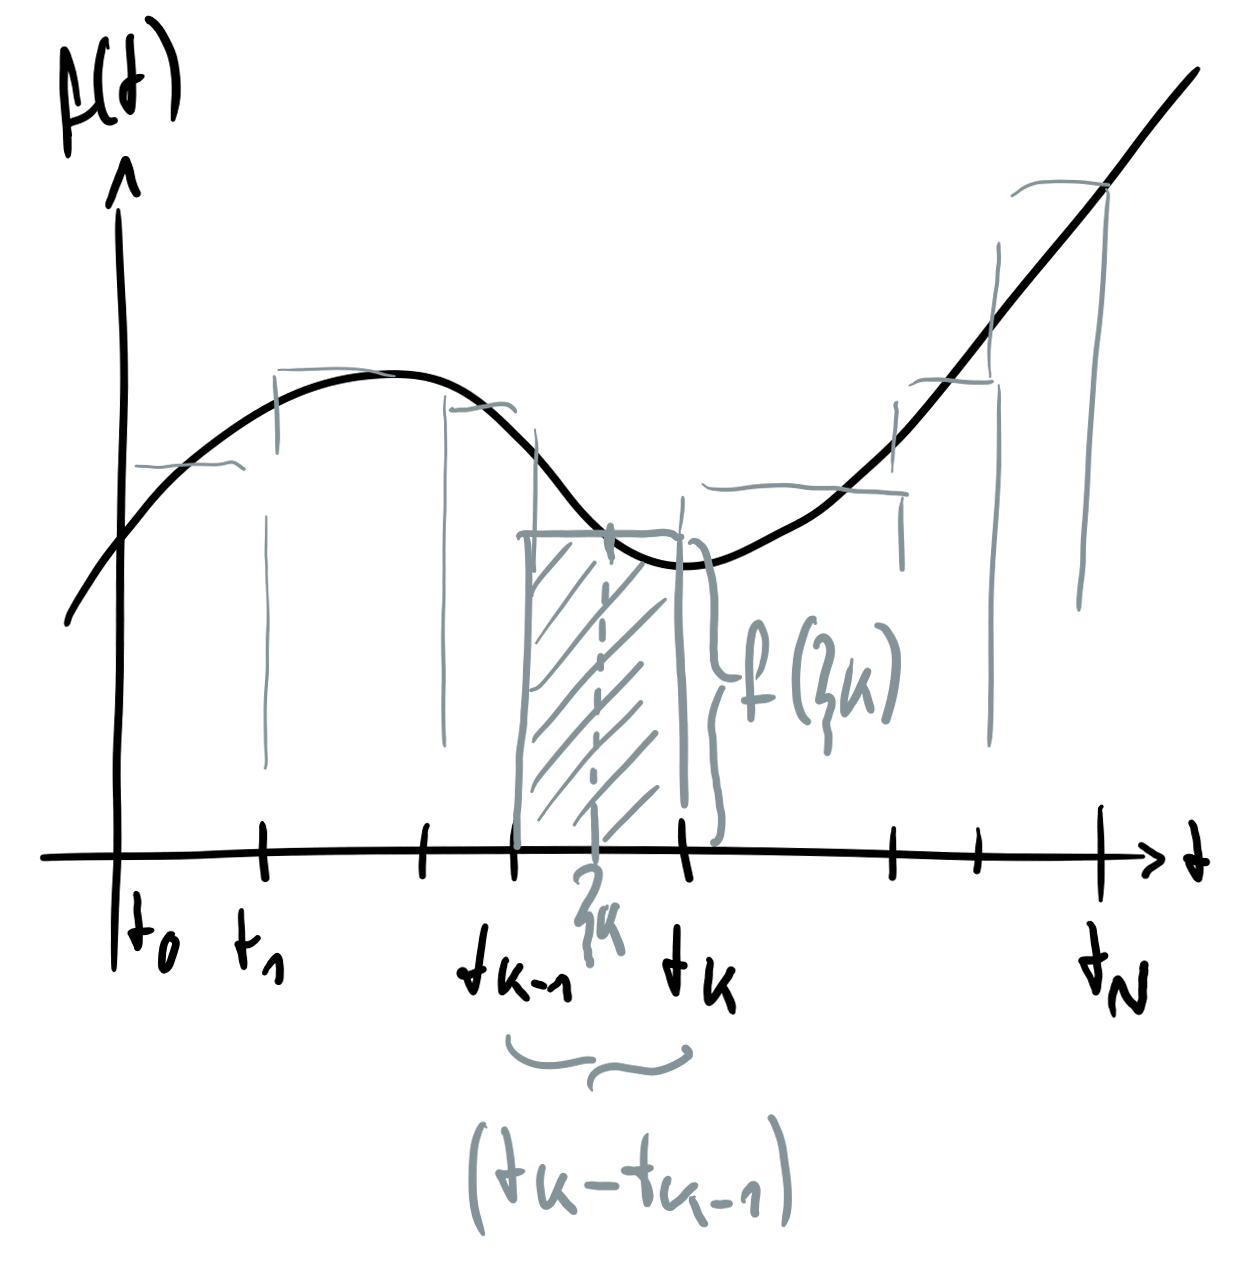
\includegraphics[width=7cm]{grafiken/Riemann-Summe.png}
  	\caption{Funktion \(f(t)\) mit Zerlegung \(t_0 < ... < t_N\) und Zwischenpunkt \(\xi_k\).}
\end{figure}

Für eine Funktion \(f: \R \rightarrow \R\) und eine Zerlegung \(a = t_0 < ... < t_n = b\) sowie beliebige Zwischenpunkte \(\xi_1, ..., \xi_n\) mit \(t_{k-1} \leqslant \xi_k \leqslant t_k\) ist die Riemann-Summe \(S(f,t,\xi\) wie folgt definiert:
\begin{align*}
	S\left(f, \left( \begin{array}{c}
		t_0 \\ \vdots \\ t_n	
	\end{array} \right), \left( \begin{array}{c}
		\xi_0 \\ \vdots \\ \xi_n	
	\end{array} \right) \right) = 
	\sum_{k=1}^n f(\xi_k)(t_k - t_{k-1})
\end{align*}
(Dabei ist \( f(\xi_k)(t_k - t_{k-1}) \) die Fläche eines Rechteckes mit Länge \(f(\xi_k)\) und Breite \( t_k - t_{k-1} \).)\\

\noindent
Weiter ist ist die Feinheit einer Zerlegung \(t=(t_0, ..., t_n)\) folgendermaßen definiert:
\begin{align*}
	\mu(t) = \max\left\{ t_k - t_{k-1}: k = 1, ..., n \right\}
\end{align*}
(Maximale Breite der unterteilten Rechtecke.)\\

\noindent
Für eine beliebige Folge \( \left( \vec{t_N} \right)_{N=1}^\infty \) von Zerlegungen mit \(\lim_{N\rightarrow\infty} \mu\left( \vec{t_N} \right) = 0\) und einer beliebigen Folge mit den Zugehörigen Zwischenpunkten \( \left( \vec{\xi_N} \right)_{N=1}^\infty \) gilt, falls der Grenzwert \( \lim_{N\rightarrow\infty} S\left( f, \vec{t_n}, \vec{\xi_N} \right)\) existiert, dann ist dieser für alle Folgen gleich und es gilt:
\begin{align*}
	\int_a^b f(t) ~dt = \lim_{N\rightarrow\infty} S\left( f, \vec{t_n}, \vec{\xi_N} \right)
\end{align*}

\subsection{Definition von Kurvenintegralen}
Gegeben sei eine Kurve \(\Kurve \subset \Rn\) und \(f : \underbrace{T(\Kurve)}_{\substack{\textrm{Träger}\\\textrm{von }\Kurve}} \rightarrow \Rn\).
\begin{enumerate}[a.~]
	\item Sei \(x: [a,b] \rightarrow \Rn\) eine Parameterdarstellung von \(\Kurve\)
	\begin{enumerate}[(i)]
		\item für eine Zerlegung \(\vec{t} : a = t_0 < ... < t_N = b\) mit zugehörigen Zwischenpunkten \(\vec{\xi} = \{ \xi_1, ... \xi_N \} \) gilt für die \textbf{Riemann(zwischen)summe}:
		\begin{align*}
			S\left( f, \vec{t}, \vec{\xi} \right) = \sum_{k=1}^N f(\xi_k) \underbrace{\cdot}_{\substack{\textrm{Skalar-}\\\textrm{produkt}}} \left(x(t_k) - x(t_{k-1})\right)
		\end{align*}
		\item Existiert ein \(I \in \R\) derart, dass für alle Folgen von Zerlegungen \(\left( \vec{t_N} \right)_{N=1}^\infty \) mit beliebigen zugehörigen Zwischenpunkten \(\left( \vec{\xi_N} \right)_{N=1}^\infty \) mit der Eigenschaft \(\lim_{N\rightarrow\infty} \mu( \vec{t_N} ) = 0\) gilt
		\begin{align*}
			\lim_{N\rightarrow\infty} S\left( f, \vec{t_N}, \vec{\xi_n} \right) = I = \int_a^b f \cdot ~dx = \int_a^b f\left( x(t) \right) \cdot ~dx(t)
		\end{align*}
		Dabei heißt \(I\) das \textbf{Kurvenintegral} von \(\Kurve\) längs \(f\).
	\end{enumerate}
	\item Existiert ein \(I \in R\) wie in (ii) so heißt \(f\) längs \(\Kurve\) \textbf{(Riemann)integrierbar} und man schreibt
	\begin{align*}
		I = \int_\Kurve f = \int_\Kurve f(x) \cdot ~dx = \int_\Kurve f_1(x) ~dx_1 + f_2(x) ~dx_2 + ... + f_n(x) ~dx_n
	\end{align*}
\end{enumerate}

\subsection{Substitutionsformel}
\label{sec:subst_formel}
Ist \(\Kurve : x(t), a \leqslant t \leqslant b\) eine stückweise differenzierbare Kurve im \(\Rn\) und \(f : T(\Kurve) \rightarrow \Rn\) stetig, dann gilt:
\begin{align*}
	\int_\Kurve f(x) \cdot ~dx = \int_a^b f(x(t)) \cdot \dot{x}(t) dt
\end{align*}
\Beweis[Beweisidee]
	\begin{align*}
		&\textrm{Nach 1ter Mittelwertsatz } \exists~\tilde{\xi}_k \in [t_{k-1},t_k]: \quad
		x(t_k) - x(t_{k-1}) = \dot{x}(\tilde{\xi}_k) (t_k - t_{k-1}) \\
		&S\left( f, \vec{t}, \vec{\xi} \right) = 
		\sum_{k=1}^N f(\xi_k) \cdot \left(x(t_k) - x(t_{k-1})\right) \stackrel{\textrm{1ter MWS}}{=} 
		\sum_{k=1}^N f(\xi_k) \cdot \dot{x}(\tilde{\xi}_k) (t_k - t_{k-1})
	\end{align*}
	Im allgemeinen gilt \(\xi_k \neq \tilde{\xi_k}\). Also wird \(\vec{\xi}\) gerade so gewählt, dass gilt:
	\begin{align*}
		S\left( f, \vec{t}, \vec{\xi} \right) = 
		\sum_{k=1}^N f\left( \underbrace{x \left(\overbrace{t_k}^{\xi_k}\right)}_{\tilde{\xi}_k}\right) \cdot \left(x(t_k) - x(t_{k-1})\right) &\stackrel{\textrm{1ter MWS}}{=} 
		\sum_{k=1}^N f(x(t_k)) \cdot \dot{x}(\tilde{\xi}_k) (t_k - t_{k-1}) \\
		&\quad \Rightarrow \quad \int_a^b f(x(t)) \cdot \dot{x}(t) ~dt
	\end{align*}
\QED
\Bemerkung Theoretisch können so die meisten Kurvenintegrale ausgerechnet werden. In der Praxis ist diese Methode aber meist nicht praktikabel.

\subsection{Beispiele}
\begin{enumerate}[(i)]
	\item Kurvenintegrale sind verallgemeinerte eindimensionale (Riemann-)Integrale. Sei \(f : [a,b] \rightarrow \R \) (eindimensionales Vektorfeld) und \(x(t) = a + t(b - a)\) (eine Kurve im \(\R^1\))
	\begin{align*}
		\int_\Kurve f = \int_\Kurve f(x) \cdot dx 
		&\stackrel{\ref{sec:subst_formel}}{=} 
		\int_0^1 f(x(t)) \cdot \dot{x}(t) ~dt \\
		&= 
		\int_0^1 f\left(\underbrace{a + t(b-a)}_{x}\right)\cdot \underbrace{(b-a) dt}_{dx} = \int_0^1 f(x) ~dx
	\end{align*}
	\item Die Länge einer Kurve kann mit einem Kurvenintegral berechnet werden. Sei \(\Kurve : x(t), a \leqslant t \leqslant b\) mit \(x\) stellenweise differenzierbar und \(\dot{x}(t) \neq 0 ~\forall~ t \in [a,b]\)
	\begin{align*}
		\int_a^b \frac{\dot{x}(t)}{\Vert \dot{x}(t) \Vert} \cdot dx(t) 
		&\stackrel{\ref{sec:subst_formel}}{=} 
		\int_a^b \frac{\dot{x}(t)}{\Vert \dot{x}(t) \Vert} \cdot \dot{x}(t) ~dt \\
		&= \int_a^b \frac{\Vert \dot{x}(t) \Vert^2}{\Vert \dot{x}(t) \Vert} ~dt = \int_a^b \Vert \dot{x}(t) \Vert = l(\Kurve)
	\end{align*}
\end{enumerate}

\subsection*{Kurvenintegrale 1. Art}
Sei \(\Kurve : x(t), a \leqslant t \leqslant b\) eine Kurve und sei \(f : \Rn \rightarrow \R\) ein stetiges Skalarfeld, dann ist das Kurvenintegral \textbf{erster} Art definiert durch:
\begin{align*}
	\int_\Kurve f(x) \cdot dx = \int_a^b f(x(t)) ~\Vert \dot{x}(t) \Vert ~dt
\end{align*}
\begin{figure}[!h]
  	\centering
 	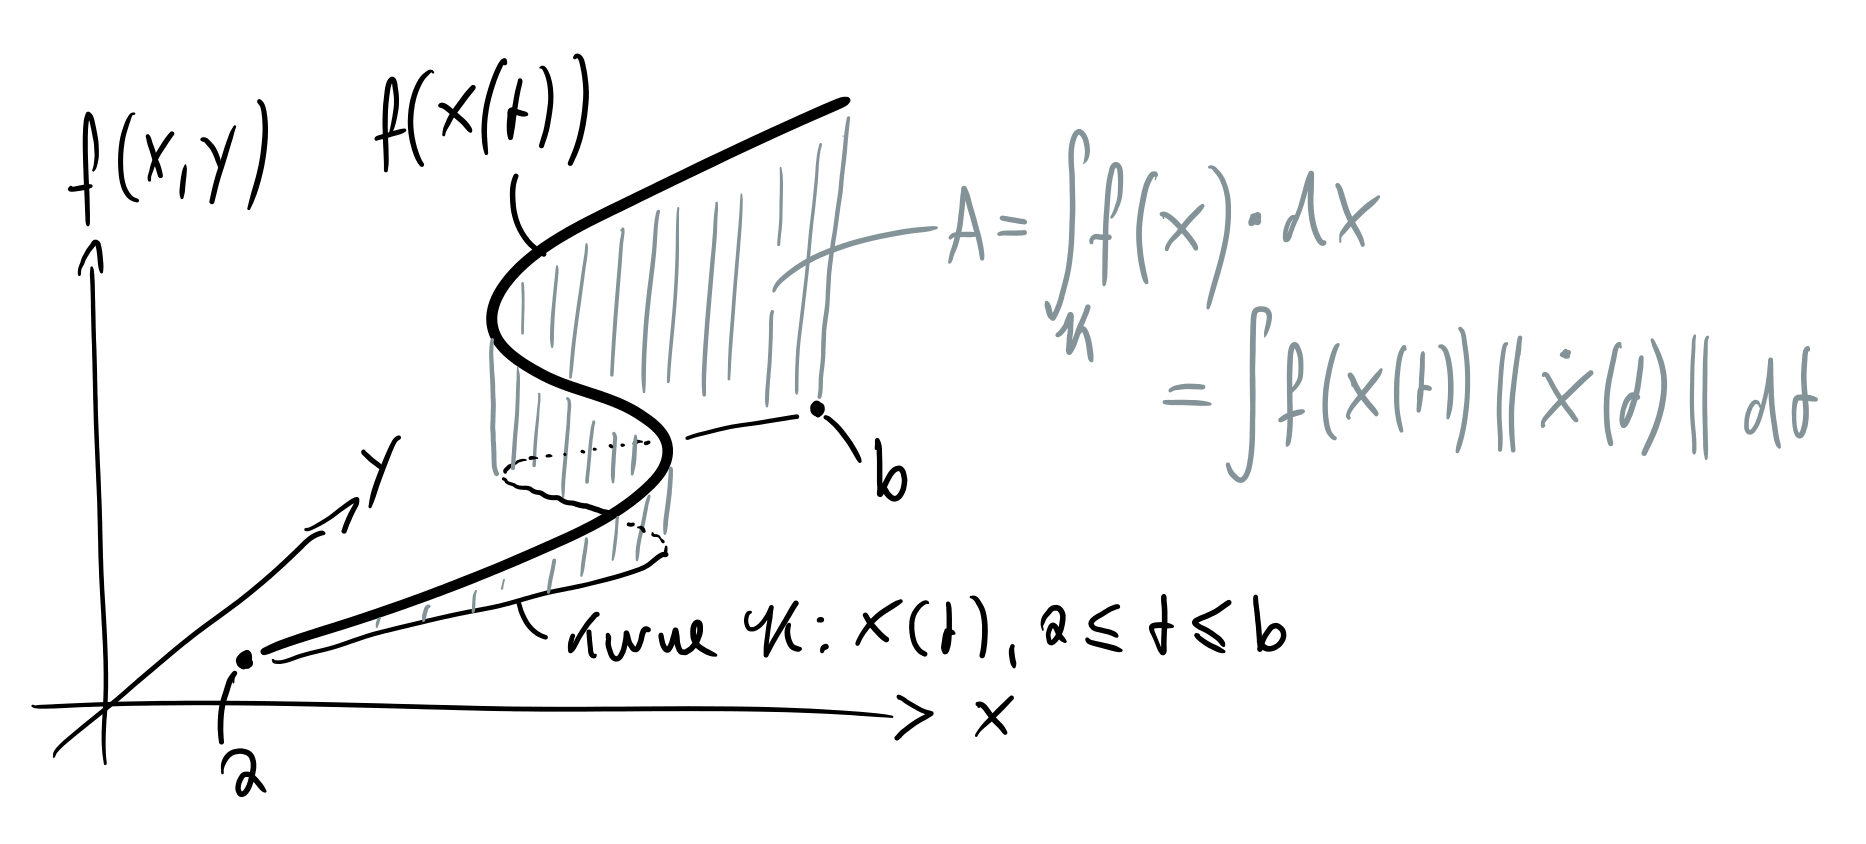
\includegraphics[width=10cm]{grafiken/Kurvenint_erster_Art.png}
  	\caption{Kurvenintegral über eine Skalarfeld \(f:\Rzwei \rightarrow \R\) erster Art.}
\end{figure}

\subsection*{Kurvenintegral 2. Art}
Sei \(\Kurve : x(t), a \leqslant t \leqslant b\) eine Kurve und sei \(f : \Rn \rightarrow \Rn\) ein stetiges Vektorfeld, dann ist das Kurvenintegral \textbf{zweiter} Art definiert durch:
\begin{align*}
	\int_\Kurve f(x) \cdot dx = \int_a^b f(x(t)) \cdot \dot{x}(t) ~dt
\end{align*}
\begin{figure}[!h]
  	\centering
 	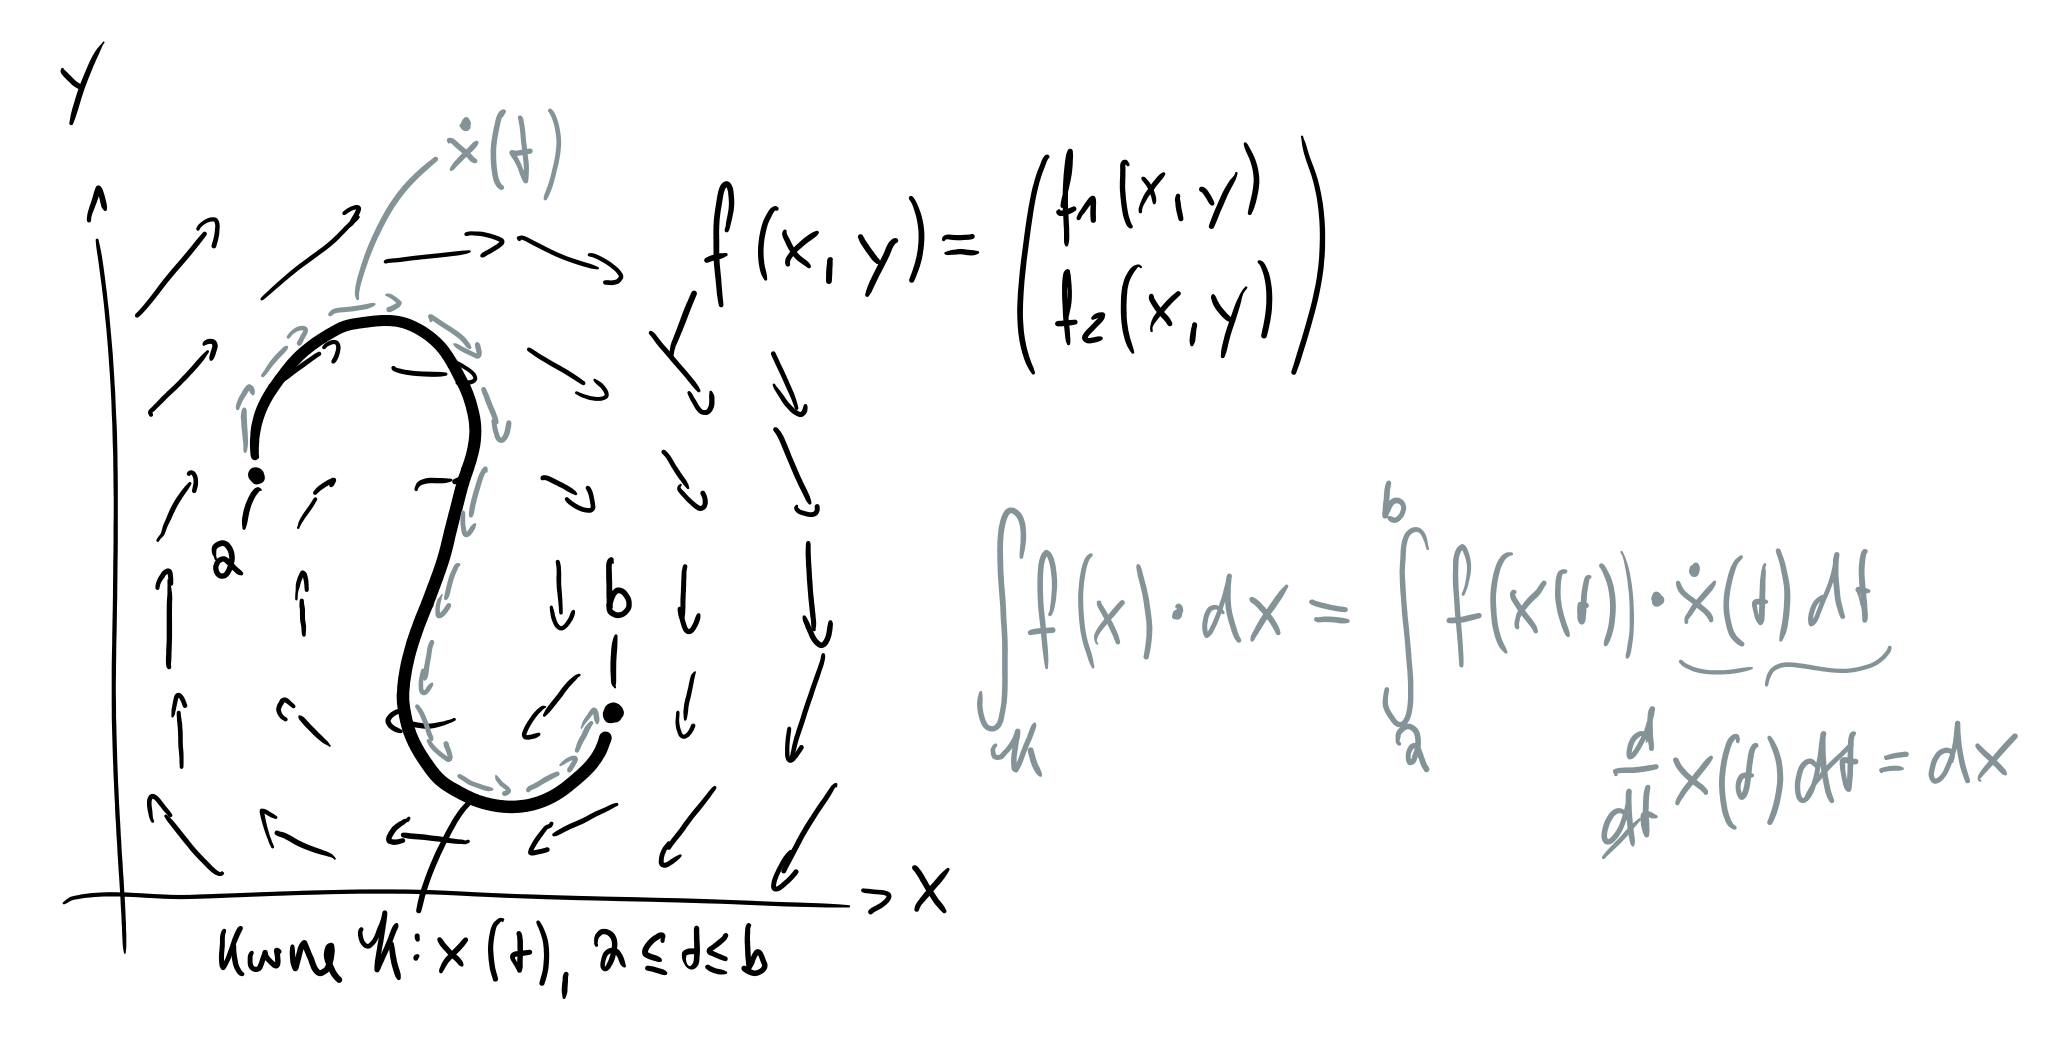
\includegraphics[width=10cm]{grafiken/Kurvenint_zweiter_Art.png}
  	\caption{Kurvenintegral über eine Vektorfeld \(f:\Rzwei \rightarrow \Rzwei\) zweiter Art.}
\end{figure}

\subsection{Definition der Wegunabhängigkeit}
Sei \(f \in C(G,\Rn), G \subset \Rn\) ein Gebiet.
\begin{enumerate}[(i)]
	\item Gilt für zwei beliebige Wege \(\Kurve\) und \(\mathcal{L}\) in \(G\) mit gleichem Anfangs- und Endpunkt stets \(\int_\Kurve f = \int_\mathcal{L} f\) dann heißt das Kurvenintegral \textbf{wegunabhängig}.
	\item Existiert eine Funktion \(F:G \rightarrow \R\) mit \(F' = \nabla F = f\) (implizit wird \(F\) differenzierbar gefordert) auf \(G\), dann heißt \(F\) eine \textbf{Stammfunktion} von \(f\).\\
	\Bemerkung In der Praxis wird das Potential eines Vektorfeldes als \(P = -F\) definiert.
	\item Ein Vektorfeld \(f\) heißt \textbf{konservativ} wenn eine Stammfunktion \(F\) in \(G\) existiert.
\end{enumerate}

\subsection{Erster Hauptsatz für Kurvenintegralen}
\label{sec:HS_kurvenint}
Sei \(f\) konservativ in \(G\) und \(F\) eine Stammfunktion, dann gilt für jeden Weg \(\Kurve\) in \(G\) mit Anfangspunkt \(p\) und Endpunkt \(q\)
\begin{align*}
	\int_\Kurve f = F(q) - F(p)
\end{align*}
Also ist insbesondere das Kurvenintegral wegunabhängig.

\Beweis (o.B.d.A. nur für glatte Kurven) Sei \(\Kurve : x(t), a \leqslant t \leqslant b\) glatt, dann gilt
\begin{align*}
	\int_\Kurve f &= \int_\Kurve f(x) \cdot dx \stackrel{\ref{sec:subst_formel}}{=}
	\int_a^b \underbrace{f(x(t))\cdot\dot{x}(t)}
	_{\substack{
		= F'(x(t))\cdot\dot{x}(t) \\
		= \frac{d}{dt} F(x(t))
	}} ~dt =
	\int_a^b \left( \frac{d}{dt} F(x(t)) \right)~dt \\
	&= \left[ F(x(t)) \right]_a^b \stackrel{\substack{\textrm{Hauptsatz}\\\textrm{der Diff/Int-}\\\textrm{Rechnung}}}{=} F(x(b)) - F(x(a)) = F(q) - F(p)
\end{align*}
\QED

\subsection{Satz}
Für \(f \in C(G;\Rn), G \subset \Rn\) ein Gebiet, sind folgende Aussagen äquivalent:
\begin{enumerate}[(i)]
	\item \(\int_\Kurve f\) ist wegunabhängig
	\item \(f\) besitzt eine Stammfunktion \(F\)
	\item \(\int_\Kurve f = 0\) für jede geschlossene Kurve
\end{enumerate}
\Beweis[Beweisansätze]\\
(ii) \(\Rightarrow\) (i): folgt direkt aus dem ersten Hauptsatz \ref{sec:HS_kurvenint}\\
(i) \(\Leftrightarrow\) (iii): Seien \(\Kurve\) und \(\mathcal{L}\) zwei Kurven mit gleichen Anfangs- und Endpunkt. So kann eine neue geschlossene Kurve \(\mathcal{M}\) wie folgt konstruiert werden:
\begin{align*}
	\int_\mathcal{M} f = \int_\Kurve f + \int_{-\mathcal{L}} = \int_\Kurve f - \int_{\mathcal{L}} = 0
\end{align*}
\QED

\subsection{Beispiele}
\begin{enumerate}[(i)]
	\item \(f(x) = \frac{x}{\Vert x \Vert^3}\) mit \(x = \left(\begin{array}{c} x_1 \\ x_2 \end{array}\right) \in G = \Rzwei \setminus \{0\}\) ist konservativ mit Stammfunktion \(F(x) = \frac{1}{\Vert x \Vert}\) ...
	\item \(f(x_1, x_2) = \left( \begin{array}{c} 2x_1x_2 \\ x_1^2 \end{array}\right)\) ist konservativ mit \(F(x_1,x_2) = x_1^2x_2\) ...
\end{enumerate}

\subsection{Definition einfach zusammenhängender Gebiete}
Ein Gebiet \(G \subset \Rn\) heißt \textbf{einfach zusammenhängend}, wenn sich jede geschlossene Kurve in \(G\) innerhalb von \(G\) \textit{stetig auf einen Punkt zusammenziehen} lässt.\\
\textit{Beispiele im \(\R^3\)}:
\begin{enumerate}[(i)]
	\item Berliner ohne Füllung ist einfach zusammenhängend.
	\item Ein Donut ist es nicht.
\end{enumerate}

\subsection{Sternförmige Gebiete}
Eine Menge \(G \subset \Rn\) heißt \textbf{sternförmig} (bezüglich einem \(x_0 \in G\)), wenn zu jedem \(x \in G\) die Strecke \(\overline{x_0 x} \subset G\) ist (komplett im Gebiet liegt).

\subsection{Bemerkung}
\begin{enumerate}[(i)]
	\item Eine sternförmige Menge ist stets auch eine einfach zusammenhängende Menge.\\
	Ein sternförmiges Gebiet ist stets auch ein sternförmiges Gebiet.
	\item Die Vereinigung von sternförmigen Gebieten muss nicht sternförmig sein.
	\item Oft kann ein einfach zusammenhängendes Gebiet als Vereinigung von sternförmigen Gebieten betrachtet werden.
\end{enumerate}

\subsection{Zweiter Hauptsatz für Kurvenintegralen}
Sei \(f \in C^1(G;\Rn)\) und \(G\) ein Gebiet, dann gilt:
\begin{enumerate}[(i)]
	\item (notwendige Bedingung) Besitzt \(f\) eine Stammfunktion \(F\) in \(G\), so erfüllt \(f\) in \(G\) die \textbf{Integrabilitätsbedingung}:
	\begin{align*}
		\frac{\partial f_k}{\partial x_l} = \frac{\partial f_l}{\partial x_k} \quad \textrm{in } G \quad \forall~ l,k \in \{1, ..., n\}
	\end{align*}
	\item (hinreichende Bedingung) Ist \(G\) einfach zusammenhängend, so besitzt \(f\) eine Stammfunktion \(F\) in \(G\), wenn die Integrabilitätsbedingung erfüllt ist.
\end{enumerate}
\Beweis[Beweisidee]
Wenn \(f\) eine Stammfunktion \(F\) hat, so muss der Satz von Schwarz gelten, also muss die Hessematrix symmetrisch sein.
\QED

\subsection{Definition der Rotation}
Sei \(G \subset \R^3\) ein Gebiet und \(f: G \rightarrow \R\) partiell differenzierbar, dann heißt die Funktion \(\textrm{rot} f : G \rightarrow \R^3 \) \textbf{Rotation} von \(f\) in \(G\) und ist folgendermaßen definiert: 
\begin{align*}
	\underbrace{\textrm{rot} f}_{\textrm{curl} f}(x) = 
	\left( \begin{array}{c}
		\frac{\partial f_3}{\partial x_2} - \frac{\partial f_2}{\partial x_3} \\
		\frac{\partial f_1}{\partial x_3} - \frac{\partial f_3}{\partial x_1} \\
		\frac{\partial f_2}{\partial x_1} - \frac{\partial f_1}{\partial x_2}
	\end{array} \right) = \vec{\nabla} \times \vec{f}
\end{align*}
\Bemerkung Die Rotation gibt an ob ein Feld Wirbel enthält.

\subsection{Korollar zum zweiten Hauptsatz für Kurvenintegrale}
Sei \(f \in C^1(G;\R^3)\) mit \(G\) ein Gebiet.
\begin{enumerate}
	\item \(f\) besitzt eine Stammfunktion \(\quad\Rightarrow\quad \textrm{rot} f = 0\) 
	\item Ist \(G\) einfach zusammenhängend, dann gilt:\\
	\(f\) besitzt eine Stammfunktion \(\quad\Leftrightarrow\quad \textrm{rot} f = 0\)
\end{enumerate}


\Bemerkung Zentralkraftfelder (wie z.b. Gravitationsfelder) haben keine Rotation und sind somit wegunabhängig.

\subsection*{Zwei Methoden zur Berechnung von Stammfunktionen:}
\subsection{Nach Variablen integrieren}
\textit{Beispiel}: Sei \(f(x,y,z) = \left(\begin{array}{c}
	y~e^{yz} + 1 \\
	x~e^{yz} + xyz~e^{yz} \\
	xy^2~e^{yz} + \cos z
\end{array} \right) = \left( \begin{array}{c}
	f_1(x,y,z) \\
	f_2(x,y,z) \\
	f_3(x,y,z)
\end{array} \right) \)\\
Gesucht ist ein \(F\) mit \(\nabla F = \left( \begin{array}{c}
	F_x \\ F_y \\ F_z
\end{array} \right) = \left( \begin{array}{c}
	f_1 \\ f_2 \\ f_3
\end{array} \right)\)
\begin{align*}
	\textrm{\underline{1.}}\quad & 
	F(x,y,z) \stackrel{!}{=} \int f_1(x,y,z) ~dx = xy~e^{yz} + x + c(y,z) \\
	\textrm{\underline{2.}}\quad & 
	F_y(x,y,z) = x~e^{yz} + xy~e^{yz}~z + 0 + c_y(y,z) \stackrel{!}{=}
	f_2(x,y,z) = x~e^{yz} + xyz~e^{yz} \\
	&\Rightarrow c_y(y,z) = 0 \quad\Rightarrow\quad c(y,z) = \tilde{c}(z) \\
	&\Rightarrow F(x,y,z) = xy~e^{yz} + x + \tilde{c}(z) \\
	\textrm{\underline{3.}}\quad &
	F_z(x,y,z) = 0~e^{yz} + xy~e^{yz}~y + 0 + \tilde{c}_z(z) \stackrel{!}{=}
	f_3(x,y,z) = xy^2~e^{yz} + \cos z \\
	&\Rightarrow \tilde{c}_z(z) = \cos z \quad\Rightarrow\quad
	\tilde{c}(z) = \int \cos z ~dz = \sin z + c \quad\mitt c \in \R \\
	&\Rightarrow F(x,y,z) = xy~e^{yz} + x + \sin z + c
\end{align*}

\subsection{Mittels Kurvenintegral und passendem Weg}
Sei \(F(x)= \int_{\Gamma_x} f\), dabei ist \(\Gamma\) ein Weg von \(x_0\) (fest) nach \(x\) in \(G\).\\

\noindent
\textit{Beispiel}: Sei \(f(x,y) = \left( \begin{array}{cc}
	- \frac{y}{x^2 + y^2} &
	\frac{x}{x^2 + y^2}
\end{array} \right)\) mit \(G = \Rzwei \setminus \left\{ \left( \begin{array}{c} x \\ 0 \end{array}\right) : x \leqslant 0 \right\}\) (sternförmig)
\begin{align*}
	\textrm{Sei}: \quad & 
	\Gamma_1 = \left( \begin{array}{c} 
		t \\
		0
	\end{array} \right), \quad
	\Gamma_2 = r \left( \begin{array}{c} 
		\cos \phi \\
		\sin \phi
	\end{array} \right)
	\quad\textrm{und}\quad x_0 = \left( \begin{array}{c}
		1 \\ 0	
	\end{array} \right) \\
	\textrm{Es gilt}: \quad & 
	F(x,y) = \int_{\Gamma_1} f + \int_{\Gamma_2} f \\
	&\qquad = 
	\int_1^r f(t,0) ~d\left( \begin{array}{c}
		t \\ 0	
	\end{array} \right) +
	\int_0^\phi f(r \cos t, r \sin t	) ~d
	\left( \begin{array}{c}
		r \cos t \\
		r \sin t
	\end{array} \right) \\
	&\qquad = 
	\int_1^r \left( \begin{array}{cc}
		-\frac{0}{t^2 + 0^2} & 
		\frac{t}{t^2 + 0^2}	
	\end{array} \right) 
	\left( \begin{array}{c}
		\frac{d}{dt} t \\
		\frac{d}{dt} 0
	\end{array} \right)\\
	&\qquad\quad + 
	\int_0^\phi \left( \begin{array}{cc}
		-\frac{r \sin t}{r^2 \cos^2 t + r^2 \sin^2 t} & 
		\frac{r \cos t}{r^2 \cos^2 t + r^2 \sin^2 t}
	\end{array} \right)
	\left( \begin{array}{c}
		\frac{d}{dt} r \cos t \\
		\frac{d}{dt} r \sin t
	\end{array} \right) \\
	& \qquad = 
	\int_1^r \left( \begin{array}{cc}
		0 & t
	\end{array} \right)
	\left( \begin{array}{c}
		1 \\
		 0
	\end{array} \right)~dt + 
	\int_0^\phi
	\left( \begin{array}{cc}
		-\frac{1}{r} \sin t & \frac{1}{r} \cos t
	\end{array} \right)
	\left( \begin{array}{c}
		-r \sin t \\
		r \cos t
	\end{array} \right)~dt \\
	& \qquad = 
	\int_1^r 0\cdot 1 + t \cdot 0 ~dt+ \int_0^\phi \frac{1}{r} \sin t \cdot r \sin t + \frac{1}{r} \cos t \cdot r \cos t ~dt \\
	& \qquad = 
	\int_1^r 0 ~dt + \int_0^\phi \frac{r}{r} \left( \cos^2 t + \sin^2 t \right)~dt =
	\int_1^r 0 ~dt + \int_0^\phi 1 ~dt \\
	\Rightarrow \quad & F(x,y) = \phi = \textrm{arg}(x,y)
\end{align*}


\end{document}








